Here we will present wavefront propagation with the unmodified Hershberger-Suri 
algorithm in mind. The only different in the regards to the modifies Hershberger-
Suri, is the sources of the wavefronts, can been sub-edges modified algorithm, 
instead of points in the unmodified.

When the conforming subdivision has been constructed we are ready to actually 
simulate the continuous Dijkstra method, by propagating through the grid with 
a wavefront expanding at a unit-speed spreading among the obstacles. At simulation 
time $t$, we say that a wavefront consists of all the points whose shortest-path
distance to the source is $t$. See figure \ref{fig:wavefrontpropagation}. Such a 
wavefront is a set of disjoint paths and closed cycles. Each path or cycle is a 
sequence of circular arcs, called \textit{wavelets}. Each of these wavelets are 
centered on a obstacle vertex that is covered by the wavefront. These vertices 
are called \textit{generators} of the wavelets. This is the reason that figure 
\ref{fig:wavefrontpropagation} has multiple sources, since if both the dashed 
and dotted arches had source at $s$, their paths from $s$ to $g$ would overlap 
(the same for $s$ to $g'$). The obstacle vertices $g$ and $g'$ are engulfed by 
the wavefront with source $s$, and becomes generators for their own wavelets.

\begin{figure}
	\centering
	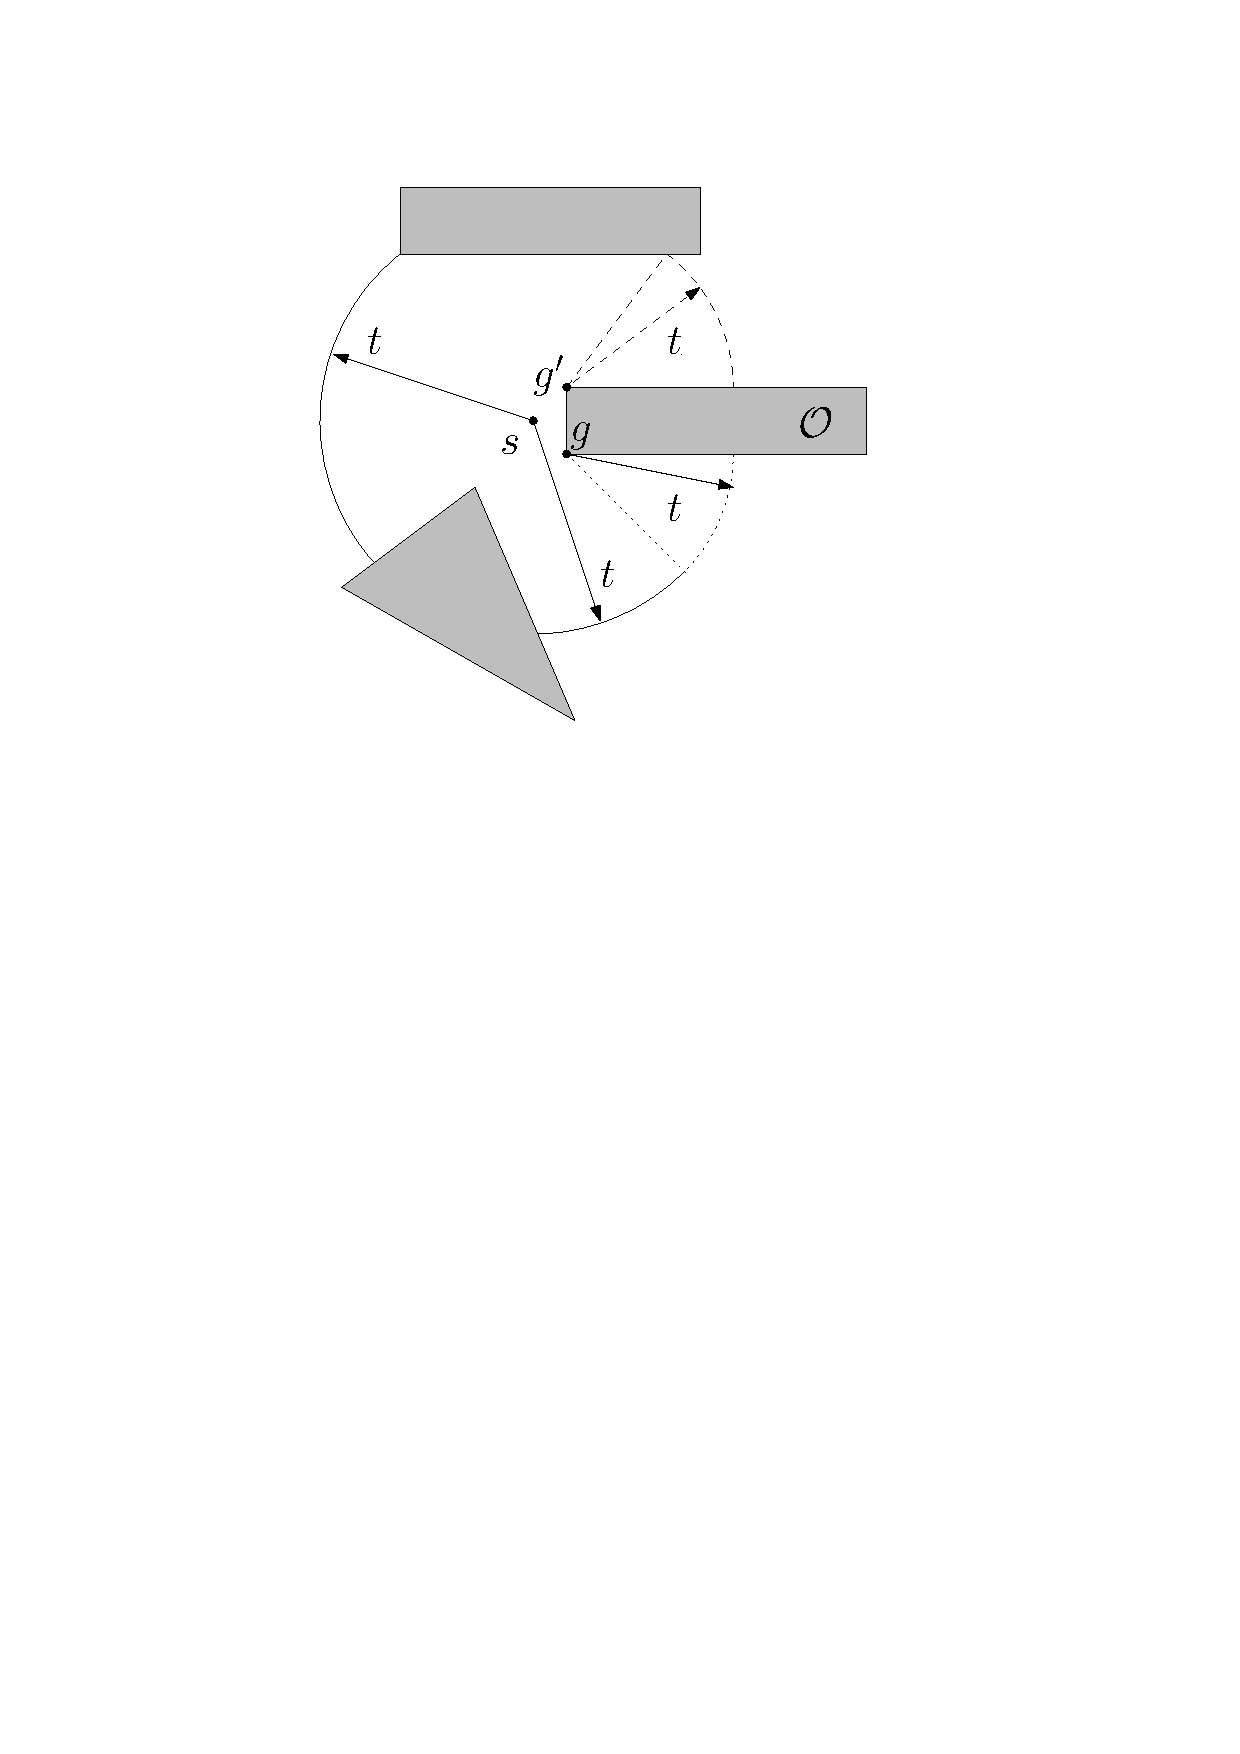
\includegraphics[width=0.45\textwidth]{figures/wavefrontpropagation.pdf}
	\caption{An example of a wavefront propagation from $s$ with distance $t$ to all
    		 points of its circular arch. Since a path into the dashed and dotted 
             area would require a turn at $\mathcal{O}$, these areas are propagated 
             by $g$ and $g'$. Since we look at the propagation at time $t$ both 
             generator would have propagated a distance $t$.}
	\label{fig:wavefrontpropagation}
\end{figure}

As the wavefront expands, the meeting point of two adjacent wavelets sweeps along a 
\textit{bisector curve}, and divides the area between them with a hyperbolic bisector 
of the two wavelets generators\footnote{see appendix A}. These ideas can be seen on 
figure \ref{fig:bisectorex}. Here $g$ and $g'$ are generators, who each starts a 
wavelet marked by the dotted line. These two wavelets meets, and for every point they 
meet, the shortest distance from this point has equal length to both $g$ and $g'$. 
This is what creates the horizontal line between $g$ and $g'$, which is the 
hyperbolic bisector. The wavefronts creates paths, which have their endpoints when 
the wavelet meet obstacles, or the planes outer boundary. These endpoints sweeps 
along the obstacle boundaries as the wavefront expands. 

From the above we see that the topology, or "shape", of wavefronts during the 
simulation changes in the case of two different event: wavefront-wavefront collisions 
 and wavefront-obstacles collisions. 

\begin{figure}[H]
	\centering
	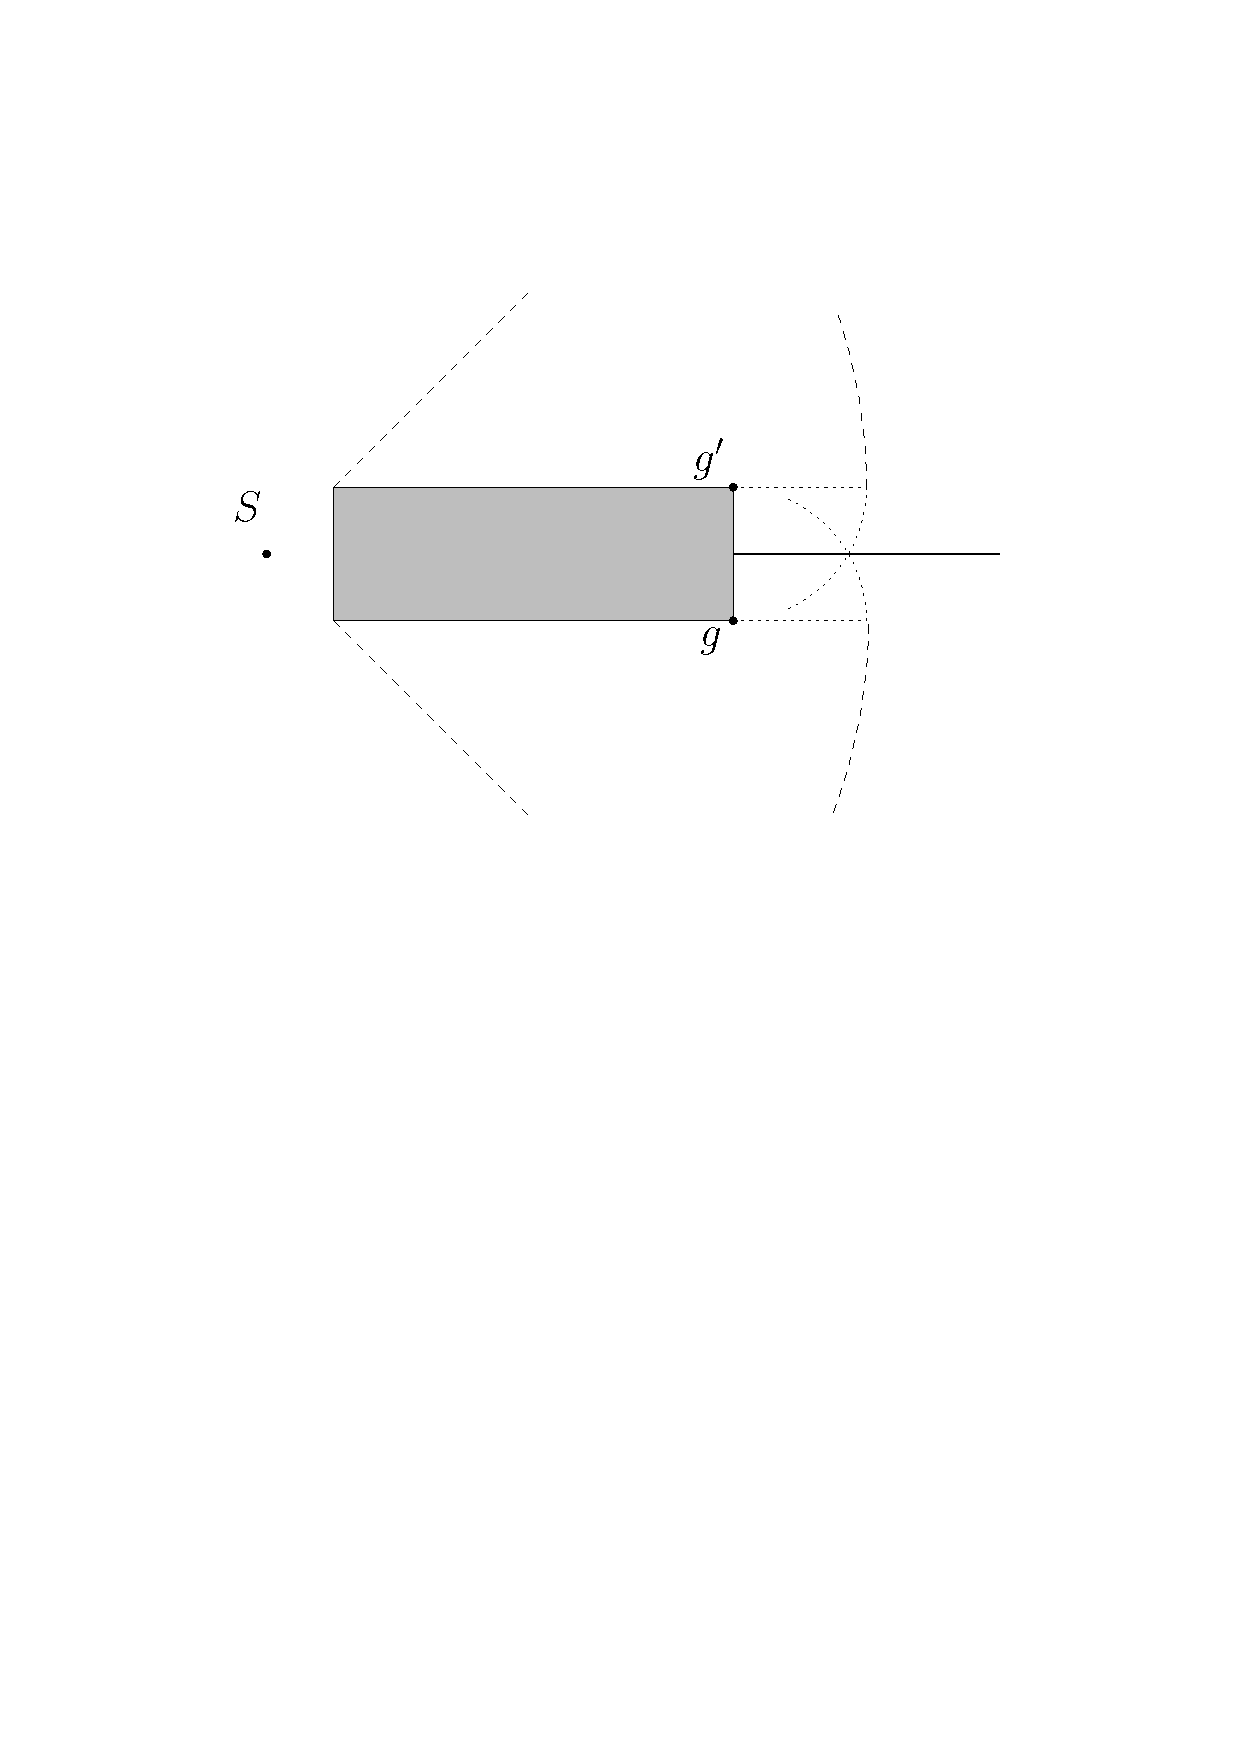
\includegraphics[width=0.45\textwidth]{figures/bisectorex.pdf}
	\caption{The adjacent generator $g$ and $g'$ each produce a wavelets which propagates 
    the space, these are represented by the dotted circular arcs. These will overlap, 
    and the split the area between them into two equal sized regions. The fully drawn 
    line segment between, then represent the splitting point between the two generators, 
    where any point on the line segment, has equal length shortest path to both of the 
    generators.}
	\label{fig:bisectorex}
\end{figure}

\section{Overview of propagation algorithm}

The wavefront propagation algorithm operates in two phases: first a wavefront 
propagation phase, and second a map computation phase. The wavefront propagation 
phase, simulates the wavefront, and thereby determines the approximate locations of 
the different wavefront collision events. We remind that there are two different kind 
of wavefront collisions, the first being the collisions where wavelets are neighbors 
in the wavefronts, that is adjacent wavelets. The second being collisions between non-
neighboring wavelets. This propagation happens through adjacent cells, and only across 
their transparent edges. We remind the reader that transparent edges are the edges 
established by the subdivision, and opaque edges, are the edges of the obstacle 
polygons. The map computation phase uses the information of wavefront collisions to 
build a shortest path map in each cell in the conforming subdivision. 

One of the main idea behind the algorithm, is the idea of calculating two 
"\textit{single-sided}" approximations of the wavefront at each transparent edge. This 
idea comes from the fact that literally translating the idea of wavefront propagation  
into an implementation would be very hard. Instead we are contempt with calculating 
for each transparent edge, two \textit{approximate wavefronts}, which will pass 
through the transparent edge, one from each side. So the job of the wavefronts is to 
assign an value $t$ to each point $p$ on an transparent edge. Here $t$ is the time it 
takes to travers at unit speed from the source $s$ to $p$. Each $p$ would have two 
such values, one from each side, where the minimum or these would the one we would use 
for a shortest path. In some cases we determine if a portion of a wavelet $w$ arrives 
after the wavelet $w'$ from the other side has fully engulfed an edge, that there is 
no need to record the time of $w$ since it is so much later than $w'$. This is also a 
reason why we refer to it as approximate, since the approximate wavefront might not 
necessarily give a complete view of all wavelets time to an edge.

\subsection{Definitions and terminology for propagation algorithm}

The following subsection borrows heavily from \cite{HershbergerS99} section 4.1 in 
terminology. We also present lemmas and proofs from this section to show correctness 
and for completeness \\

By visiting the cells in a correct order, and going cell by cell we can calculate the 
correct time in which a wavefront hits a transparent edge, within a giving 
approximation which will be enough for our purpose. To do that we formalize the 
following to sets of edges for an edge $e$, $input(e)$ and $output(e)$.

By $input(e)$ we mean the set of edges whose approximate wavefronts we use when computing 
the approximate wavefront collision with $e$, and as such the distance to $e$. This set 
consists of transparent edges on the boundary of $\mathcal{U}(e)$ which is the well covering 
region of $e$. This is described in section \ref{section:def-well-covering-if-regions}.
Computing the approximate wavefront at $e$ then consist of propagating the approximate 
wavefronts from $input(e)$ to $e$ inside $\mathcal{U}(e)$. It is quite clear that a shortest 
path without violation only needs to bend in the case getting around an obstacle, and the 
same is true for the wavefront. Because $\mathcal{U}(e)$ neither needs to convex, or even 
simply connected, nonconvexity of $\mathcal{U}(e)$ can block the wavefronts from some edges 
of $input(e)$ from reaching $e$. Typically, paths corresponding to blocked wavefronts either 
pass through free space outside $\mathcal{U}(e)$ and re-enter through other edges of 
$input(e)$ of simply run into obstacles outside $\mathcal{U}(e)$. 

By $output(e)$ we refer to the set of edges where $e$ influences the approximate wavefront. 
Formally we define $output(e)$ as 

$$output(e) = input(e) \cup \{ f | e \in input(f) \}$$

The reason $output(e)$ contains $input(e)$ is the algorithm is depending on $output(e)$ 
having a cyclic enclosing of $e$ for detecting wavefront collision events.

\begin{Lemma}[Lemma 4.1 in \cite{HershbergerS99}] \label{lemma:4.1} \hspace{1cm} \\
For any transparent edge $e$, $output(e)$ contains a constant number of edges.
\end{Lemma}
\begin{proof}
	Due to $|\mathcal{U}(f)| = O(1)$ for all edge $f$, and each $\mathcal{U}(f)$ being a 
    connected set of cells of $\mathcal{S}'$, no edge $e$ can belong to $input(f)$ for more 
    than $O(1)$ edges $f$.
\end{proof}

The implementation of the wavefront propagation is loosely synchronized. A main idea of 
approximate wavefront propagation being approximate lies in the following implementation: 
For a transparent edge $e=\overline{ab}$ we define 

$$\tilde{d}(s,e)=\min(d(s,a),d(s,b))$$ 

This estimates $d(s,e)$ because if the wavefront hits $a$ or $b$ then $\tilde{d}(s,e) = 
d(s,e)$, with $d(s,e)$ being the real distance from $s$ to $e$. Should the wavefront hit 
right in the middle, between the endpoints of $\overline{ab}$, then the distance to $a$ and 
$b$ from the point the wavefronts collides with would be $\title{d}(s,e)=d(s,e)+\frac{1}
{2}|e|$. Since if we, in the later case, move the point of collision in any direction the 
distance becomes smaller, since it must hold that $d(e,s) \leq \tilde{d}(e,s) \leq d(e,s) + 
\frac{1}{2}|e|$. 

Since we want to compute the covering time of each $e$, i.e. the time at which $e$ is 
completely covered by the wavefront. We set the time to $\tilde{d}(s,e)+|e|$. It is 
obviously a conservative estimate of when the whole edge is fully covered. This time can 
easily be calculated on the fly and only be looking at the $input(e)$. We denote the time 
where the edge $e$ is fully covered by $covertime(e)$. 

\subsection{The propagation algorithm, main loop}

Initially we look at every $e$ that is in the well-covering region $\mathcal{U}(e)$ (which 
also includes the source point $s$). We proceed to calculate an upper bound on $\tilde{d}
(s,e)$ considering only straight-line paths inside $\mathcal{U}(e)$ and set the 
$covertime(e) = \tilde{d}(s,e) + |e|$. For all other edges $e$ we initialize $covertime(e) = 
\infty$. This implies if the $covertime(e)$ is set to $\infty$, then the shortest path 
$\pi(s,a)$ or $\pi(s,b)$ must exit the boundary of $\mathcal{U}(e)$.

The algorithm for simulation, maintains a time parameter $t$ and processes each edge in 
order of its covertime. The main loop of the simulation is as follows:

\begin{algorithm}[H]
	\caption{Propagation Algorithm} \label{algorithm:propagationalgorithm}
	\begin{algorithmic}[1]
		\While {there is an unprocessed transparent edge}
        	\State Select edge $e$ with minimum $covertime(e)$
            \State Set time $t$ to $covertime(e)$
            \State \multiline{compute the approximate wavefronts at $e$ 
            		based on the approximate 
        		    wavefronts from all edges $f\in input(e)$ satisfying 
                    $covertime(f) < covertime(e)$}
            \State Compute $d(v,s)$ exactly for each endpoint $v$ of $e$.
            \ForEach {edge $g \in output(e)$}
           		\State \multiline{Compute time $t_g$ when approximate wavefront 
                	   from $e$ first engulfs an endpoint of $g$}
                \State Set $covertime(g)$ to $\min(covertime(g), t_g + |g|)$.
            \EndFor
        \EndWhile
	\end{algorithmic} 
\end{algorithm}

Lemma \ref{lemma:4.2} provides a proof of the propagation algorithms consistency, by showing 
$covertime()$ is correctly maintained and the edges needed for processing $e$ would already have 
been processed. 

\begin{Lemma}[Lemma 4.2 in \cite{HershbergerS99}]\label{lemma:4.2}
During the wavefront propagation the following invariants hold:

\begin{enumerate}[(a)]
	\item If a wavefront of an edge $f \in input(e)$ contributes to an
	approximate wavefront of e then $\tilde{d}(f,s)+|f|<\tilde{d}(e,s)+|e|$.
	\item The value of $covertime(\cdot)$ is updated a constant number of times.
	\item The final value of $covertime(e)$ is $\tilde{d}(e,s)+|e|$. This value
	is reached no later than the simulation clock reaches that time.
%side 16
	\item Edge e is processed at simulation time $\tilde{d}(e,s) + |e|$
	\end{enumerate}
\end{Lemma}

\begin{proof} 
The parts of the lemma are proven individually

	(a) If a wavelet is able to contribute to the approximate wavefront at $e$
	it must be the case that it reaches $e$ at some time $t_e$ where $d(e,s) \leq
	t_e \leq \tilde{d}(e,s)+|e|$. 
	On the way from $s$ to $e$ the wavelet either goes straight from $s$ in side 
	$\mathcal{U}(e)$ or by going through another transparent edge  $f \in inpute(e)$ at an 
    earlier time $t_f$ 
	with $d(s,f) \leq t_f < \tilde{d}(s,f)+|f|$ and $t_e \geq t_f+d(f,e)$.  
	Since we know from $(W3_{fs})$ of a well-covering region with parameter 2, 	   
    $d(f,e)\geq 2|f|$	
	and so $t_e \geq d(s,f)+2|f|$. Since $\tilde{d}(s,f)+\frac{1}{2}|f|$, it
	must be the case that $\tilde{d}(s,f)+|f|<\tilde{d}(s,e)+|e|$. \\

	(b) The value of $covertime_e$ is only updated when an edge $f$ is processed
	from either $f \in input(e)$ or $e \in input(f)$. There are $O(1)$ such edges by
	Lemma \ref{lemma:4.1} \\

	(c),(d) These are proven by induction on the simulation clock. (c) and
	(d) holds for the edges $e$ whose initial $covertime_e$ values are not
	infinite. The wavelets that first reaches an endpoint of $e$, at
	$t_e=\tilde{d}(s,e)$ passes through some $f \in input(e)$. Because of the
	base-case in the induction we know that $f$ has has already been visited before the 
    simulation clock
	reaches $t_e$ and so $covertime_e$ is set to $\tilde{d}(s,e)+|e|$ no later
	than $t_e=\tilde{d}(e,s)$. The variable $covertime_e$ cannot be set to any
	smaller value, because no approximate wavefront can reach the endpoints of
	$e$ earlier than $\tilde{d}(s,e)$. It follows that $e$ will be processed at
	simulation time $\tilde{d}(s,e)+|e|$.
\end{proof}

\begin{Lemma}[Lemma 4.3 in \cite{HershbergerS99}]
	For every vertex v of our conforming subdivision, the propagation algorithm
	correctly determines the distance $d(s,v)$ before $v$ is used as a generator in
	any wavefront.	
\end{Lemma}

\begin{proof}
	In the conforming subdivision, every vertex $v$ is an endpoint of a transparent edge 
    $e$. The wavefront that creates the distance $d(s,v)$, either reaches $v$ by only 
    traveling within the boundary of $\mathcal{U}(e)$ or exists through an edge $f \in 
    input(e)$ s.t. $covertime(f) < covertime(e)$. The case of not leaving $\mathcal{U}(e)$, 
    the initialization trivially computes $d(s,v)$ correctly. The case of leaving 
    $\mathcal{U}(e)$, step 4 and 5 in algorithm \ref{algorithm:propagationalgorithm} 
    implies $d(s,v)$ would be correctly computed. Should $v$ be an obstacle vertex, it may 
    appear as a generator in a wavefront, but it will not be used until $d(s,v)$ is 
    computed at time $\tilde{d}(s,e)+|e|$ (Lemma \ref{lemma:4.2} (d))
\end{proof}

Even though a well-covering region $\mathcal{U}(e)$ has constant complexity, it might not be 
a simply connected component. One could consider the case of a square annulus. Consequently 
there might be multiple topologically distinct paths from a boundary edge $f \in input(e)$ 
to $e$. But we're not interested in comparing paths of different topologies, so to avoid 
comparisons of different topological paths we split the wavefront $W(e)$ into topologically 
equivalent pieces. 

For this purpose, let $W(e)$ denote one of the approximate wavefront passing through $e$. Now 
when we will compute $W(e)$ from the set $\{W(f)|f \in input(e)\}$, we will use topologically 
constrained versions of the two incoming wavefronts, which we will denote $W(f,e)$. In this 
context a wavefront $W(f,e)$ will be a portion of $W(f)$ that follows a single topological 
path inside $\mathcal{U}(e)$ from $f$ to $e$.

To further extend this notation, we can consider a $\mathcal{U}(e)$ which contains holes. 
In this cell there will therefore be multiple topologically distinct paths from an edge $f 
\in input(e)$ to $e$. When distinguishing between the multiple topologically different 
wavefronts from a single edge $f$ to $e$, we will use a primed notation $W(f,e)$, $W(f',e)$ 
etc.

Lets assume that two point $p, q \in e$ are hit by a single topologically constrained 
wavefront $W(f,e)$. The segment of $e$ which has $p$ and $q$ as endpoints then all of the 
segments points has among their predecessor the generator vertices in $W(f)$, which 
intersects $f$ and $f$. Also the quadrilateral bounded by the segments of $f$ and $e$, which 
is a subset of $\mathcal{U}(e)$. Such paths are not always segments. We can imaging an 
obstacle vertex $v$ which lies in a well-covering region of $e$, and the path from $f$ to $p$ 
turns at $v$. This would then imply that the predecessor of $p$ in $W(f,e)$ may be $v$. 
Should this be the case, then the paths from $p$ and $q$ to $f$ can be continuously deformed 
(there is no obstacles between the two paths) to each inside $\mathcal{U}(e)$. 

Unless $s \in \mathcal{U}(e)$, then for any points $p \in e$ the shortest path $\pi(s,p)$ 
would pass through some $f \in input(e)$, an so constrain the source wavefronts to pass 
through $input(e)$, and by doing so not lose any essential information for the path.

\subsection{The artificial wavefronts}

As mentioned earlier, conceptually when calculating the distance to a transparent edge $e$, we 
can get to situation where one wavefront will consume the edge way before the other edge even 
reaches $e$. In such a situation we would want to discard the wavefront arriving later, 
because we don't need it. The concept for this the artificial wavefronts. This mechanism will 
also be our only mechanism for pruning the wavefront that arrives second at a transparent 
edge. The easiest way to understand artificial wavefronts is by an example, see figure 
\ref{fig:artificialwavefront} below.

\begin{figure}[H]
	\centering
	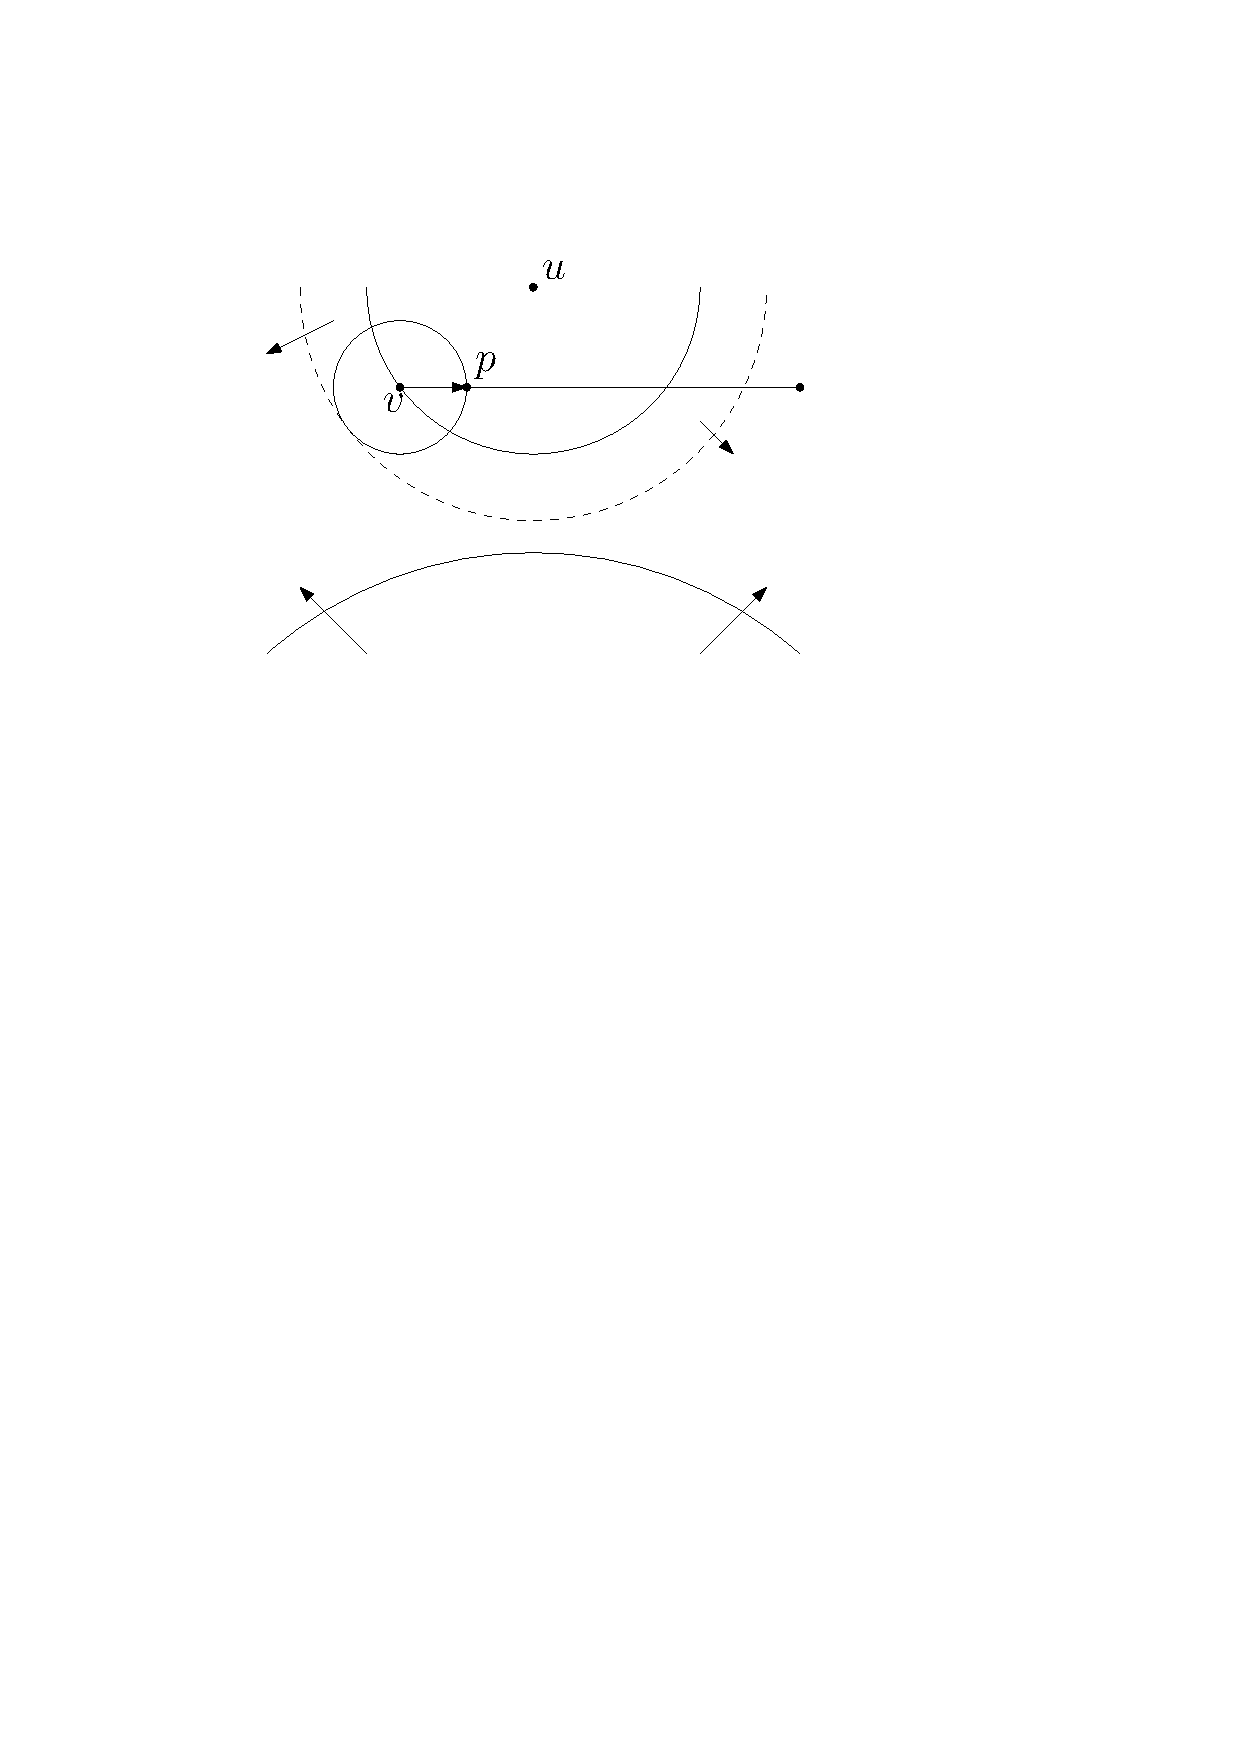
\includegraphics[width=0.45\textwidth]{figures/artificialwavefront.pdf}
	\caption{An example of an artificial wavefront from $v$ reaching point $p$ on edge $e$}
	\label{fig:artificialwavefront}
\end{figure}

Here $u$'s wavefront engulfs the left side of the transparent edge below it, lets call it $e$. 
The left endpoint of $e$ is $v$. When we is engulfed $v$ will generate a artificial wavefront, 
which will run along $e$. In the figure we see that $v$ artificial wavefront engulfs $p$ 
before the wavefront from the other side even reaches $e$. By the triangular inequality we 
have $d(s,p) \leq d(s,v) + |\overline{vp}|$ for any point $p \in e$. This surely means that 
the upper wavefront reaches $p$ first, and there is therefore no need to continue the 
propagation of the lower wavefront through $p$.

So when computing the approximate wavefront passing through $e$ from below, the contributing 
wavefronts are the following:

\begin{enumerate}
\item All wavefront $W(f,e)$ for $f \in input(e)$ and $f$ below the line supporting $e$. As 
mentioned before, we differentiate between paths of topological difference, so if $f$ 
intersect the line supporting $e$, we then split $W(f,e)$ into two, and keep only the portion 
$W(f',e)$ that comes from the part of $f$ below $e$.
\item An artificial wavefront expanding from each endpoint of $e$. These generator, e.g. $v$ 
from figure \ref{fig:artificialwavefront} has weight $d(v,s)$.
\end{enumerate}

So in essence, the artificial wavefront is a convenient mechanism for discarding parts the 
actual wavefront which will be completed dominated by other parts of the wavefront. Since we 
only use the artificial wavefront to discard parts of incoming wavefronts, their generators 
will not be passed on to $output(e)$ as part of the approximate wavefront, unless it's also a 
vertex of $\mathcal{O}$.

%%%%%%%%%%%%%%%%%%%%%%%%%%%%% what to do with this %%%%%%%%%%%%%%%%%%%%%%%%%%

\subsubsection{Proof for artificial wavefronts}

The following proofs are taken from \cite{HershbergerS99}, and included for completeness.

Consider a set of wavefronts that reach $e$ from the same side. We say that a
contributing wavefront $W(f)$  claims a point $p \in e$ if $W(f)$ reaches $p$
before any other contributor from the same side of $e$.

\begin{Lemma}[Lemma 4.4] 
	Let $e$ be horizontal  and let W(f,e) and W(g,e) be two contributors to the
	approximate wavefront that passes through e from below. Let x and x' be
	points on e claimed by W(f,e) and let y be a point e claimed by W(g,e). The
	y cannot lie between x and x'.
\end{Lemma}
\begin{proof}
	Consider the the shortest paths $\pi(x,s)$, $\pi(x',s),$ and $\pi(y,s)$ in
	the modified enviroment in which $e$ has been replaced by an open, opaque
	segment. These paths connect $x$ and $x'$ to $f$ and $y$ too $g$, inside
	$\mathcal{U}(e)$. Shortest paths $\pi(x,s)$, $\pi(x',s),$ and $\pi(y,s)$ do
	not cross. The subpaths of $\pi(x,s)$ and $\pi(x',s)$ inside
	$\mathcal{U}(e)$ can be continuously deformed to each other inside
	$\mathcal{U}(e)$, so $g$ is not between them. It follows that $y$ is not
	between them, either.
\end{proof}
\begin{Lemma}[Lemma 4.5]
	Let u and v be two obstacle vertices, both generating wavelets that are
	considered when the approximate wavefront passing through an edge e from
	below is computed. Then the bisector generated by u and v intersects e at
	most once in SPM(s).
\end{Lemma}
\begin{proof}
	Suppose the bisector intersects $e$ twice. Without lose of generality assume
	$u$ lies inside the loop formed by the bisector and $e$. If the bisector
	intersects $e$ twice in $u$ lies inside the loop formed by the bisector and
	$e$. If the bisector intersects $e$ twice in $SPM(s)$, then the segment from
	$u$ to its predecessor must intersect $e$ between the two bisector
	intersections.  The means that $d(e,s)<d(u,s)$, in fact, $d(e,s)+2|e|\leq
	d(u,s)$. Hence $\tilde{d}(e,d)+|e| < d(u,s)$ and $u$ cannot contribute to
	the approximate wavefront at $e$: it does not become a generator until after
	$e$ is prcoessed, contradicting the assumption that both $u$ and $v$
	contribute to the approximate wavefront at $e$.
\end{proof}

\begin{Lemma}[Lemma 4.6] \label{lemma:4.6HersherbergerS99}
	Given $w(f,e)$	for each f below e that contributes to $W(e)$ we can compute
	the interval of e claimed by each $W(f,e)$ in $O(1+k)$ total time, where $k$
	is the total number of generators in all wavefronts $W(f,e)$ that are absent
	from $W(e)$.
\end{Lemma}

\begin{proof}
	For each contributing wavefront $W(f,e)$, we show how to determine the
	portion of e claimed by $W(f,e)$ if only one other contributing wavefront
	$W(g,e)$ is present. Lemma 4.4 implies that this portion is contiguous. The
	intersection of these  claimed portions taken over all other contributors
	$W(g,e)$, is part of $e$ claimed by $W(f,e)$ in $W(e)$.

	In constant time we determine whether the claim of $W(f,e)$ is left or right
	of that of $W(g,e)$. If both $W(f,e)$ and $W(g,e)$ reach the left endpoint
	of $e$ in constant time, check which one reaches it sooner. Otherwise one of
	$W(f,e)$ and $W(g,e)$ reaches a point on $e$ that is left of any point
	reached by the other, and this point determines the ordering. Without loss
	of generality, assume that the claim of $W(f,e)$ is left of that of $W(g,e)$

	By Lemma 4.4 we can combine the two wavefronts using only local operations.
	Let $a$ denote the generator in $W(f,e)$ claiming the rightmost point on
	$e$. Let $p_a$ be the left endpoint of $a$'s interval on $e$. Similarly, let
	$b$ denote the generator in $W(g,e)$ claiming the leftmost point on $e$ and
	let $p_b$ be the right endpoint of $b$'s interval on $e$. Compute the
	bisector of $a$ and $b$, and let its intersection with $e$ be the point $x$.
	(By Lemma 4.5 there is only one intersection poiny in $SPM(s)$. If the
	hyperbola generated by $a$ and $b$ intersects $e$ twice, then $a$ is to the
	left of $b$ at only one of the intersections, and we use that intersection
	as $x$.) See figure 4.2. If $x$ is to the left of $p_a$, then delete a from
	$W(f,e)$ if $x$ is to the right of $p_b$, then delete $b$ from $W(g,e)$ in
	either case redefine $a$, $b$, $p_a$, $p_b$ recompute $x$, and repeat this
	test. If $p_a$ is left of $p_b$ and x lies between them then $x$ is the
	right endpoint of $W(f,e)$'s claim in the presence of $W(g,e)$
	
    \begin{figure}[H]
	\centering
	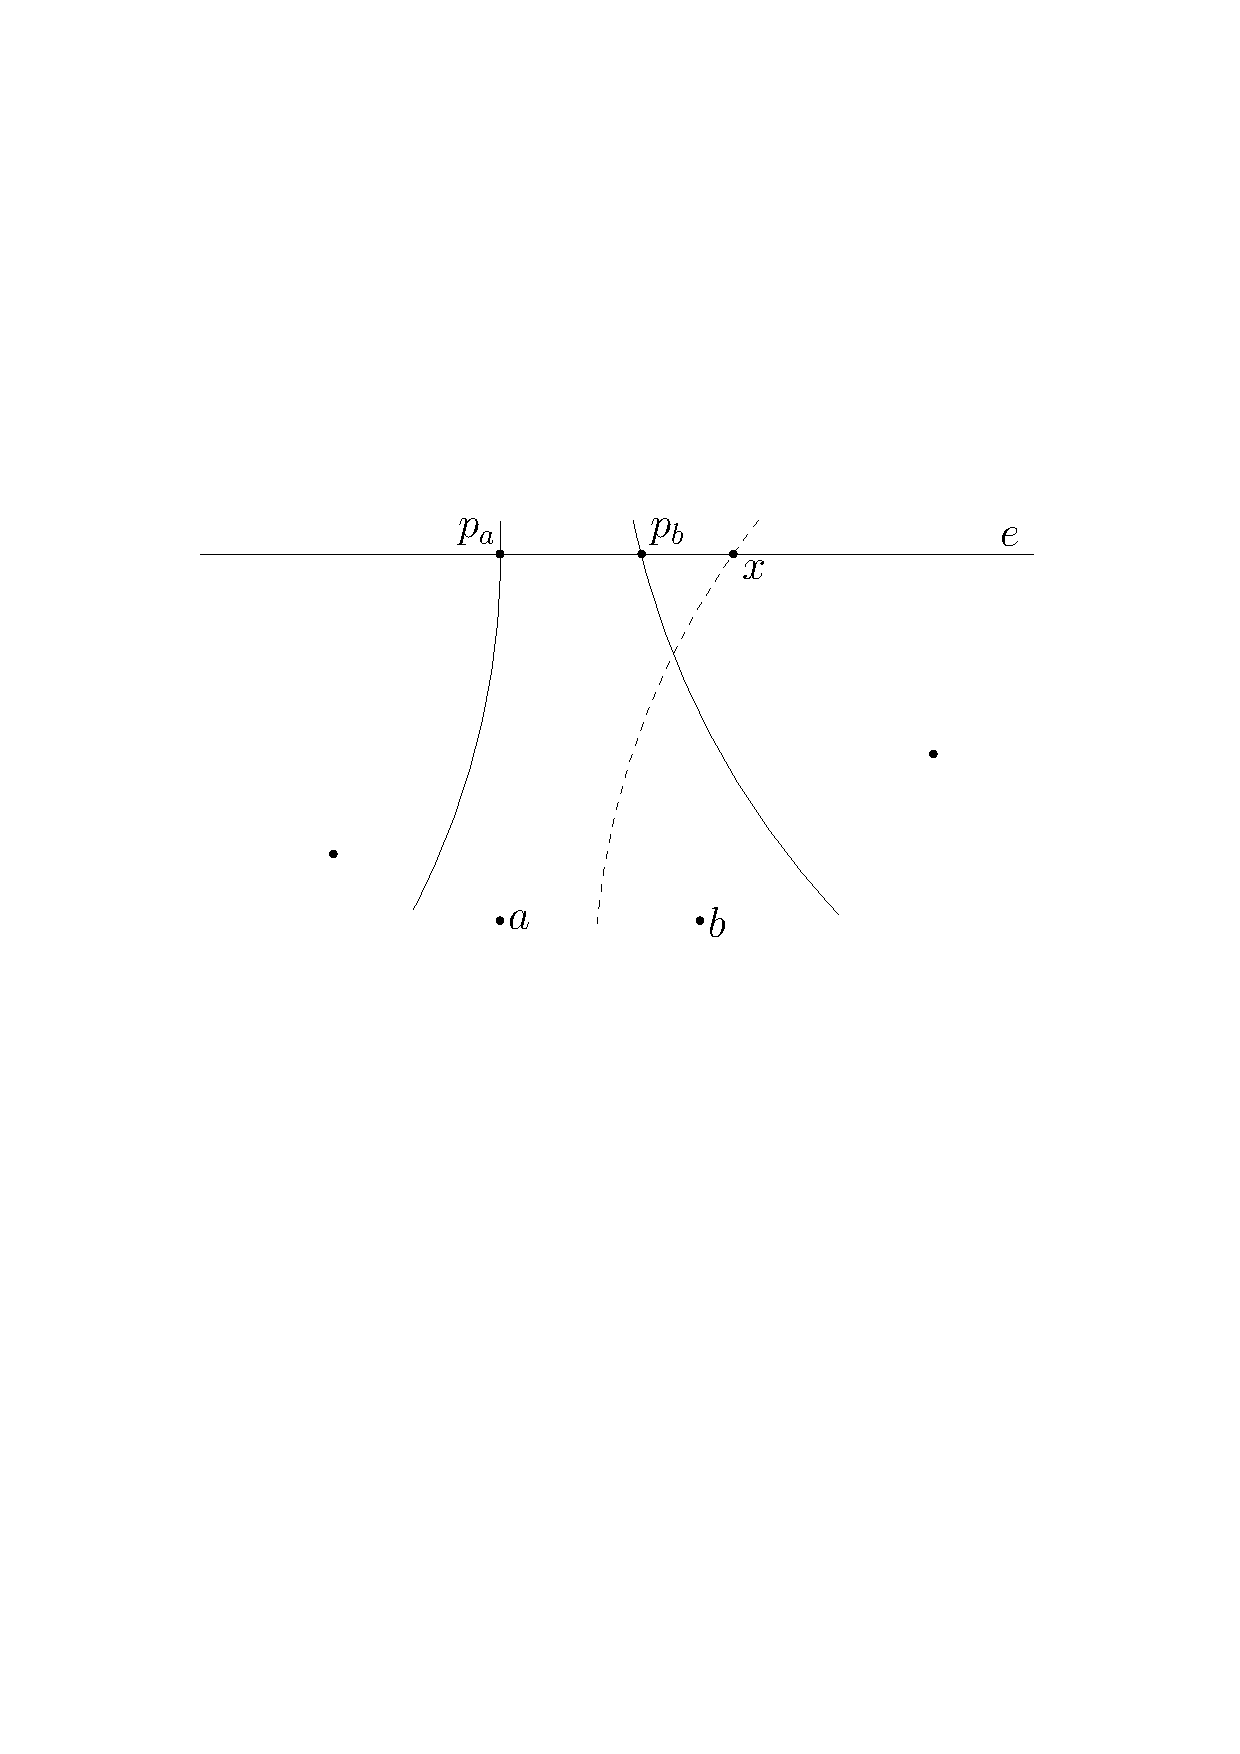
\includegraphics[width=0.65\textwidth]{figures/contribution.pdf}
	\caption{The contribution of $b$ to $W(e)$ is constrained to be left of $p_b$ 
    		 and right of $x$ and therefore does not exist.}
	\label{fig:artificialwavefront}
	\end{figure}

	By combining the claimed regions for all contributors $W(f,e)$ we construct
	the approximate wavefront $e$. The time bound follows since spend constant
	time per generator that is deleted for each pair of wavefronts, and he total
	number of wavefronts $W(f,e)$ to be merged is also constant. This finishes
	the proof
\end{proof}
\begin{Lemma}
	Any generator deleted during the construction of an approximate wavefront at
	edge $e$ does not contribute to the true wavefront at $e$. Every generator
	that contributes to the true wavefront at $e$ either is $s$ or belongs to
	one of the approximate wavefronts at $e$.
\end{Lemma}
\begin{proof}
	The first part is clear-every deleted generator is dominated by some other
	generator at $e$. The second part follows by induction from two facts: any
	wavelet that contributes to the true wavefront at $e$ must come either from
	$s$ inside $\mathcal{U}(e)$ or through one of the edges in $input(e)$ (by
	the definition of well-covering). The approximate wavefronts at $input(e)$
	are ready before they are needed to construct $W(e)$ (by Lemma 4.2)
\end{proof}

%%%%%%%%%%%%%%%%%%%%%%%%%%%%%%%%%%%%%%%%%%%%%%%%%%%%%%%%%%%%%%%%%%%%%%%%%%%%%%%%%%%%%

\subsection{The bisector events} \label{section:bisectorevents}

First we remind the reader that when we speak of bisectors, we refer to the meeting points of 
two adjacent wavelets along a bisector curve, which divides the area between them with a 
hyperbolic bisector, see figure \ref{fig:bisectorex}. When we talk about bisector events we 
mean the event of intersections of bisectors with each other or with obstacles. These may 
happen when we propagate an approximate wavefront $W(e)$ to $output(e)$. These bisector event 
may be detected in two ways:

\begin{enumerate}
\item During the computation of $W(e,g)$ from $W(e)$ for some $g \in output(e)$. This kind of 
	  bisector event is detected when simulating the propagation of wavefront from $e$ to $g$ 
      to compute $W(e,g)$. In particular, when two generators $u$ and $v$ are non-adjacent in 
      $W(e)$, but at any time in the propagation form $e$ to $g$ become adjacent, then there 
      is a bisector event involving $u$ and $v$.
      \peter{evt forklarer merging udenfor lemmaet, hvis det flyttes skal der gøre noget}
\item During the merging process described in Lemma \ref{lemma:4.6HersherbergerS99}. Let a 
	  generator $v$ be contributing to one of the input wavefronts $W(e,g)$, but not the the 
      merged wavefront $W(g)$ at $g$, then $v$ will be involved in the bisector event on the 
      way from $e$ to $g$.
\end{enumerate}

The algorithm for detecting bisector events, detects these in a small proximity to their 
actual location in $SPM(s)$. The process of doing this is by \textit{marking} the generators 
that participate in a bisector event in $O(1)$ cell near where the event is detected. So if a 
generator $v$ is involved in a bisector event in a cell $v$, then $v$ is guaranteed to belong 
to a set of marked generators for $c$. It may however be the case that the set of marked 
generators for a cell $c$ is a superset of generators that actually participate in bisector 
events in $c$. The proof of showing that this total number of generator marked in all the cell 
in $O(n)$ will be shown in Lemma \ref{lemma:4.9HershbergerS99}

We here state the rules for Marking generators as given in \cite{HershbergerS99}.

\begin{enumerate}
\item If a generator $v$ lies in a cell $v$, them mark $v$ in $c$.
\item Let $e$ be a transparent edge, and let $W(e)$ be the approximate wavefront coming from 
	  some generator $v$'s side of $e$.
      \begin{enumerate}[a]
      \item If $v$ claims an endpoint of $e$ in $W(e)$, or if it would do so except for an 
            artificial wavefront, then mark $v$ in all cells incident to the claimed endpoint.
      \item If $v$'s claim in $W(e)$ is shortened or eliminated by an artificial wavefront, 
      		then mark $v$ in the cell on $v$'s side of $e$.
      \end{enumerate}
\item Let $e$ and $f$ be two transparent edges with $f \in output(e)$. Mark $v$ in both the 
	  cells that have $e$ as an edge if one of the following event occurs:
      \begin{enumerate}[a]
      \item $v$ claims an endpoint of $f$ in $W(e,f)$;
      \item $v$ participates in a bisector event detected either during the computation of 
      		$W(e,f)$ from $W(e)$, or during the merging step at $f$. We also mark $v$ as 
            having a bisector event if $v$'s claim of $W(f)$ is shortened by an artificial 
            wavefront.
      \end{enumerate}
\item If $v$ claims part of an opaque edge when it is propagated from an edge $e$ toward 
	  $output(e)$, mark $v$ in both cells with $e$ on their boundary.
\end{enumerate}

From the above we see that both rule 2a and 3a apply when a wavefronts claims an endpoints of 
an edge $e$. The difference lies in 2a marking cells near the claimed end point while 3a puts 
marks in cells near the source edge of the wavefront.

%%%%%%%%%%%%%%%%%%%%%%%%%%%%%%%%%%% Copied from article %%%%%%%%%%%%%%%%%%%%%%%%%%%%%%%%%

\subsubsection{Proof for bisector events}

The following proofs are taken from \cite{HershbergerS99}, and are included for completeness.

A generator may contribute to a wavefront more than once in the wavefront sequence; each mark 
applies to only one instance of the generator in the sequence. The following technical lemma 
is used in the proof of Lemma \ref{lemma:4.9HershbergerS99} to establish the correctness of 
the marking rules.

\begin{Lemma}[Lemma 4.8 in \cite{HershbergerS99}] \label{lemma:4.8HershbergerS99}
	Let $v$ be a generator that contributes to an approximate wavefront $W(e)$
	suppose there i a point $p \in e$ that is claimed by $v$ in $W(e)$ but not
	in $SPM(S)$ (because a wave from the other side of $e$ reaches $p$ first)
	Then $v$ is marked in the cell $c$ on $v$'s side of $e$.
\end{Lemma}
\begin{proof}
	If $v$ is unmarked in $c$ there must be generators $u$ and $w$ such that
	$u$, $v$, $w$ are consecutive in $W(e)$ --- otherwise  Rule 2 would
	apply. The bisectors $(u,v)$ and $(v,w)$ must exit from $\mathcal{U}(e)$
	though the same transparent edge $h$ --- otherwise Rule 3 or 4 would
	apply. For the same reason, the region bounded by $(u,v)$, $(v,w)$, $h$,
	and $e$ is a subset of $\mathcal{U}(e)$ --- if th region contained a
	non-$\mathcal{U}(e)$ island, $v$ would claim an endpoint of a boundary
	edge of that island. Edge $h$ is by definition part of $input(e)$.
	Consider the point $p \in e$ that is claimed by $v$ in the approximate
	wavefront $W(e)$ but not in th true wavefront at $e$, and suppose that
	the true predecessor of $p$ is $z\neq v$. The vertex $z$ is either an
	obstacle vertex or the source $s$. In the former case, $z$ lies outside
	$\mathcal{U}(e)$ or on its boundary $\partial\mathcal{U}(e)$ --- by
	condition (C3), $\mathcal{U}(e)$ contains at most one obstacle vertex, so
	any vertex not strictly outside $\mathcal{U}(e)$ must be connected to
	points outside $\mathcal{U}(e)$ by opaque edge. Vertex $z$ may lie
	strictly inside $\mathcal{U}(e)$ only if $z=s$.

	Let us first assume that $z$ lies outside the well-covering region
	$\mathcal{U}(e)$ --- the proof simplifies in the other case, which is
	considered below. Let $q$ denote the intersection point between
	$\overline{zp}$ and $input(e)$ closet to $p$ (recall that $input(e)
	\subset output(e)$ and $input(e) \subset \partial\mathcal{U}(e))$. Based
	on the position of $q$ relative  to the bisector $(u,v)$ and $(v,w)$ we
	argue that $v$ must have been involved in a bisector event detected by
	our algorithm and thus marked in cell $c$.

	First consider the case in which $q$ lies between the bisectors $(u,v)$
	and $(v,w)$ on the edge $h$. Now, since $|\overline{qp}|\geq|h|$ (by the
	well-covering property), the endpoints of $h$ are engulfed by a wavefront
	from $z$ or from some other generator before the wavefront from $z$
	reaches $p$ at time $d(z,s) + |\overline{zp}|$. The artificial wavefront
	from $h$'s endpoints will cover $h$ before time
	$d(z,s)+|\overline{zp}|+|h|$. By assumption we have
	$d(v,s)+|\overline{vp}| > d(z,s)+|\overline{zp}|$. The wavefront from $v$
	cannot reach $e$ earlier than $d(v,s)+|\overline{vp}| - |e|$. By
	well-covering with parameter 2, $d(e,h)$ is at least $|e|+|h|$ and so the
	wavefront from $v$ reaches $h$ no earlier than
	$d(v,s)+|\overline{vp}|+|h|>d(z,s)+|\overline{zp}|+|h|$, at which time
	$h$ is already covered by the artificial wavefront. The claim of $v$ on
	$h$ is shortened by the artificial wavefront (in fact $a$'s claim is
	eliminated completely), and so it must be marked by Rule 3b.

	In the second case, $q$ is not between the bisectors $(u,v)$ and $(v,w)$
	on $h$. The segment $\overline{qp}$ must intersect one of the bisectors.
	Without loss of generality, assume $\overline{qp}$ intersects bisector
	$(u,v)$. Since every point on $\overline{qp}$ has $z$ as its predecessor
	in $SPM(s)$, the bisector $(u,v)$ does not reach $\partial\mathcal{U}(e)$
	in $SPM(s)$. We show that our propagation and merging algorithms will
	detect a bisector event for $(u,v)$. Let $r$ be the intersection point
	between the bisector $(u,v)$ and the edge $h$. As noted in the discussion
	after Lemma 4.3, the triangle defined by the segments $\overline{ur}$,
	$\overline{vr}$ and $e$ is a subset of $\mathcal{U}(e)$. Bisector $(u,v)$
	crosses the triangle boundary on $e$ and at $r$, but nowhere else. The
	larger region $R$ bounded by $e$, $h$, $\overline{ur}$ and bisector
	$(v,w)$ also is a subset of $\mathcal{U}(e)$ and it contains point $p$.
	Because $\overline{qp}$ crosses into $R$ to intersect $(u,v)$ and it does
	not intersect the $(v,w)$ or $h$ sides of $R$, $\overline{qp}$ must
	intersect $\overline{ur}$ let $x$ be the point of intersection. The
	wavelet from $z$ reaches $x$ before the one from $u$, so the path $z
	\to x \to r$ starting at time $d(z,s)$ reaches $r$ before the path $u \to
	r$ starting at time $d(u,s)$. Observe also that the path $z \to x \to r$
	is a legal path --- it lies in free space. Now, consider the shortest
	path from $z$ to $r$ inside the triangle $\bigtriangleup zxr$ that does
	not cross $h$ or any obstacle edge (see Figure 4.3). Because $z\to x \to
	r$ lies in free space, such a path exists and is shorter than $z \to x
	\to r$. This path claims $r$ from the same side as $u$ before the wavelet
	from $u$ reaches $r$. (If the path passes through an endpoint of $h$,
	then an artificial wavefront 
	%side 22
	claims $r$ otherwise the last obstacle
	vertex on the path claims $r$.) Thus a bisector event for $(u,v)$ is
	detected during the computation of $W(e,h)$ or $W(h)$ and $v$ is marked
	by Rule 3b.

	Next consider what happens if the predecessor vertex $z$ lies on the
	boundary of the well-covering $\mathcal{U}(e)$. Let $h$ be a boundary
	edge $\mathcal{U}(e)$ incident to $z$. In this case we detect a bisector
	event involving $v$ when we advance the wavefront from $e$ to
	$output(e)$: if $z$ lies between the bisectors $(u,v)$ and $(v,w)$ then
	$v$ is marked by Rule 3a or 4 if $z$ is not between the bisectors, the
	segment $zp$ intersects one of the bisectors, say $(u,v)$ and we detect a
	bisector event for $(u,v)$ in advancing the wavefront from $e$ to
	$ouput(e)$.

	Finally consider the case in which $z=s$ lies inside $\mathcal{U}(e)$. If
	$z$ is not between the bisectors $(u,v)$ and $(v,w)$ segment
	$\overline{zp}$ intersects one of them and the proof is as above. Let $r$
	be the intersection of $(u,v)$ with $h$ and let $t$ be the intersection
	of $(v,w)$ with $h$. The convex quadrilateral bounded by subsegments of
	$e$, $\overline{ur}$, $h$, and $\overline{tw}$ is contained inside
	$\mathcal{U}(e)$. Hence if $z$ is between the bisectors $(u,v)$ and
	$(v,w)$, the entire segment $\overline{rt}$ is visible from $z$ (that is
	$\bigtriangleup zrt$ is empty) and so $v$'s claim on $h$ is eliminated by
	$z$. Therefore $v$ is marked by Rule 3b. This completes the proof.

\end{proof}
\begin{Lemma}[Lemmma 4.9 in \cite{HershbergerS99}]\label{lemma:4.9HershbergerS99}
	If a generator $v$ participates in a bisector event of $SPM(s)$ in a cell
	$c$, then $v$ is marked in $c$.
\end{Lemma}
\begin{proof}
	If a bisector has an endpoint on an opaque edge of $c$, it either
	emanates from an obstacle vertex on the edge, or it is defined by two
	generators that claim part of the opaque edge. Rule 1 and 4 guarantee
	that all such generators are marked in $c$.
	If a generator $v$ that contributes to an approximate wavefront in $c$ is
	unmarked then by Rule 2a there must be transparent edges $e$ and $f$ on
	the boundary of $c$ such that $W(e)$ and $W(f)$ both contain the
	generator subsequence $u$, $v$, $w$ for some $u$ and $w$.
	Without loss of generality assume $W(e)$ enters $c$ and $W(f)$ leaves
	$c$. If $v$ participates in a bisector event of $SPM(s)$ in $c$, then at
	least one point $p$ inside the region $R$ bounded by $e$, $f$, $(u,v)$
	and $(v,w)$ is not claimed by $v$ in $SPM(s)$. Let $z$ be the true
	predecessor of $p$. Let $r$ and $t$ be the intersections of $(u,v)$ and
	$(v,w)$ with $f$, respectively. Region $R$ is contained in the convex
	quadrilateral $Q$ bounded by $\overline{ur}$, $\overline{rt}$,
	$\overline{tw}$, and the line supporting $e$. Because $u$, $v$, $w$ is a
	subsequence of $W(e)$, no vertex on the same side of $e$ as $v$ claims
	any point of the side of $Q$ collinear with $e$, that is, $\overline{zp}$
	does not cross that side of $Q$. If $r$ and $t$ are both claimed by $v$
	in $SPM(s)$ then $\overline{ur}\in \pi(s,r)$ and $\overline{wt}\in
	\pi(s,t)$. In this case $\pi(s,p)$ cannot cross $\overline{ur}$ or
	$\overline{wt}$ and hence it
	%side 23
	must cross $\overline{rt}$. The intersection of $\overline{zp}$ with
	$\overline{rt}$ is a point $q$ that satisfies the hypothesis of Lemma 4.8,
	and so $v$ is marked in $c$. On the other hand if either $r$ or $t$ is not
	claimed by $v$ in $SPM(s)$ that vertex satisfies the hypothesis of Lemma 4.8
	and so $v$ is marked in $c$.
\end{proof}

The following technical lemma shows that the approximate wavefront are not too
different from the true wavefronts this lets us bound the number of marks made
by the marking rules.
\begin{Lemma}[Lemma 4.10 in \cite{HershbergerS99}] \label{lemma:4.10HershbergerS99}
	Let $B$ be the set of pairs (e,b) of transparent edges e and bisectors b
	such that b crosses e in some approximate wavefront but the same crossing
	does not occur in SPM(s). Then $|B|=O(n)$
\end{Lemma}
\begin{proof}
	Let $(e,b)$ be a pair in $B$. Bisector $b$ is defined by two generators $u$
	and $v$. The proof of Lemma 4.8 notes that each generator (except possibly
	$s$) is outside or on the boundary of $\mathcal{U}(e)$. That proof also
	shows that $b$'s intersection with $e$ in some approximate wavefront (that
	is, the presence of $u$ and $v$ in $W(e)$) is proof that $u$ and $v$ claim
	points on the boundary of $\mathcal{U}(e)$ (in $input(e)$) in $SPM(s)$. Let
	$p=b \cap e$. Because $(e,b)$ is not an incident pair in $SPM(s)$, there
	must be at least one bisector event in $SPM(s)$ that lies in the interior of
	$\mathcal{U}(e)$ between the line segment $\overline{up}$ and
	$\overline{vp}$. We can charge the early demise of $b$ to any one of these
	bisector events.

	The segments $\overline{pu}$ and $\overline{pv}$ are disjoint inside
	$\mathcal{U}(e)$ from the corresponding segments defined by any other pair
	$(e,b') \in B$ in the modified shortest path problem in which the obstacles
	are $O\cup \{e\}$ the segments $\overline{pv}$ and $\overline{pu}$ belong to
	$\pi(s,p)$ and hence they are disjoint from any other such segments. Thus
	the sector bounded by $\overline{pu}$ and $\overline{pv}$ is disjoint inside
	$\mathcal{U}(e)$ from the sector defined by any other pair $(e,b') \in B$ so
	each bisector event inside $\mathcal{u}(e)$ is charged at most once for all
	pairs in $B$ that have $e$ as the first element of the pair. Each cell in
	the conforming subdivision belongs to $O(1)$ well-covering regions
	$\mathcal{U}(e)$. Hence the sum over all transparent edges $e$ of the number
	of bisector events in $\mathcal{U}(e)$ is only $O(n)$. This total is an
	upper bound on $|B|$.
\end{proof}

\begin{Lemma}[Lemma 4.11  in \cite{HershbergerS99}] \label{lemma:4.11HershbergerS99}
	The total number of marked generators over all cells is $O(n)$
\end{Lemma}
\begin{proof}
	We begin by defining a propagation region for each edge $e$. For any
	transparent edge $e$ let $P(e)$ be the collection of cells through which
	wavefronts propagate on the way from $e$ to all edges $f \in output(e)$.
	Clearly $P(e)\subseteq \mathcal{U}(e) \cap \{\mathcal{U}(f)|f\in
	output(e)\}$. The number of cells in $P(e)$ is constant since $|output(e)|$
	is constant and so is the number of cells in $\mathcal{U}(f)$ for any $f$.
	Furthermore since every cell of $P(e)$ is within a constant number of cells
	of $e$, each cell $c$ belongs to $P(e')$ for only a constant number of edges
	$e'$.

	The total number of generator-cell marks made under Rule 1 is clearly $O(n)$

	Each $P(e)$ has constant complexity so there are $O(n)$ edge pairs $(e,f)$
	where $e$ is transparent and $f$ is either transparent and in $output(e)$ or
	opaque and inside or on the boundary of $P(e)$. From this it follows that
	the number of marks made by Rules 2a and 3a is $O(n)$. similarly there are
	$O(n)$ Rule 4 marks in which the wavelet from $v$ claims an endpoint of the
	opaque edge or is the first or last nonartificial wavelet in $W(e)$.

	Any Rule 4 mark not yet counted involves a generator $v$ that does not reach
	any opaque edge endpoint when propagated forward from $e$. Because $v$ is
	not the first or last nonartificial wavelet in $W(e)$, there is a generator
	$u$ such that $v$'s claim on $e$ in $W(e)$ is bounded on the left of
	bisector $(u,v)$. We can assume that $(u,v)$ intersects $e$ in $SPM(s)$ by
	Lemma 4.10 there are only $O(n)$ bisector-edge pairs that intersect in
	approximate wavefronts but not in $SPM(s)$. Bisector $(u,v)$ terminates in
	$P(e)$ either on the opaque edge or in a bisector event before the opaque
	edge. Let us charge the
	%Side 24
	marking of $v$ at $e$ to this endpoint of $(u,v)$ in $SPM(s)$. Because each
	cell belongs to $P(e')$ for a constant number of edges $e'$, each vertex of
	$SPM(s)$ is charged $O(1)$ times. Since $|SPM(s)|=O(n)$, the number of RULE
	4 marks is $O(n)$.

	The proof for rule 2b and 3b are similar to that Rule 4. We begin with the
	proof for Rule 3b. We can assume that the interval claimed by $v$ on $e$ in
	$W(e)$ is bounded by two bisectors $(v,u)$ and $(v,w)$ for two nonartificial
	generator $u$ and $w$ the first and last generators in $W(e)$ counted
	separately sum to at most $O(n)$ overall. Furthermore we can assume that
	$(u,v)$ and $(v,w)$ both intersect $e$ in $SPM(s)$ there are only $O(n)$
	bisector-edge pairs that appear in some approximate wavefront but not in
	$SPM(s)$ (Lemma 4.10). At least one of the two bisector fails to reach the
	boundary of $P(e)$ in $SPM(s)$ because Rule 3b applies and a detected
	bisector event implies the existence of an actual bisector event no later
	than the point of detection we charge the marking of $v$ to that bisector
	endpoint. Each bisector event gets charged $O(1)$ times and there are $O(n)$
	bisector events in $SPM(s)$.

	To bound the number of rule 2b marks, consider where the generator $v$ lies.
	There is at most one generator $v$ inside $\mathcal{U}(e)$ and so $O(n)$
	marks for such generators overall. If $v$ lies outside $\mathcal{U}(e)$
	there is at least one edge in $input(e)$ where $v$ is marked by Rule 3b
	because of the shortening of $v$'s claim on $e$. Charge the Rule 2b mark at
	$e$ to this Rule 3b mark. There are $O(n)$ Rule 3b marks and hence $O(n)$
	Rule 2b marks
\end{proof}
We defer the finer details of the propagation algorithm to section 
\ref{section:implwavefront} and instead describe the second phase of the 
algorithm next, namely the shortest path map computation.

%%%%%%%%%%%%%%%%%%%%%%%%%%%%%%%%%%%%%%%%%%%%%%%%%%%%%%%%%%%%%%%%%%%%%%%%%%%%%%%%%%%%%%

\subsection{Computing the shortest path map}

So far in this section we have gone through the propagation phase. In this phase we have 
propagate the plane with wavefronts and wavelets from generator, and we have used approximate 
wavefronts for each transparent edge to sort out dominated wavefronts. We also marked generators
in every cell $c$, where each marked generator is in the approximate wavefront of one of the 
boundary edges of $c$, an all but $O(1)$ of them contribute to a bisector event either in $c$ or 
in one of $O(1)$ nearby cells. Here the bisector event was the intersections of bisectors with 
each other or with obstacles. The sketch of an algorithm from the proof of Lemma 
\ref{lemma:4.6HersherbergerS99}, will be presented in section \ref{section:implwavefront}, which 
will let us compute the marked generators in $O(\log n)$ time a piece. 

This section is dedicated to show how we can break the interior area of a cell $c$ into 
\textit{active} and \textit{inactive} regions. This splitting will be done on the basis of 
whether a vertex of $SPM(s)$ lie in a region. If it does we denote the area as active, and if 
no vertex is present in the area we denote it as inactive. We saw in section 
\ref{section:bisectorevents}, lemma \ref{lemma:4.9HershbergerS99} that only marked generator 
would contribute to a bisector event in $c$. 

A bisector made by a marked generator and an unmarked neighbor generator will be drawn in the 
$SPM(s)$. All such bisectors are disjoint, and we will see the partition of $c$ into active 
and inactive regions, will be done such that active regions are claimed only by unmarked 
generators and inactive regions by marked generators. This can be seen in figure 
\ref{fig:activeinactiveregions}. 

\begin{figure}[H]
	\centering
	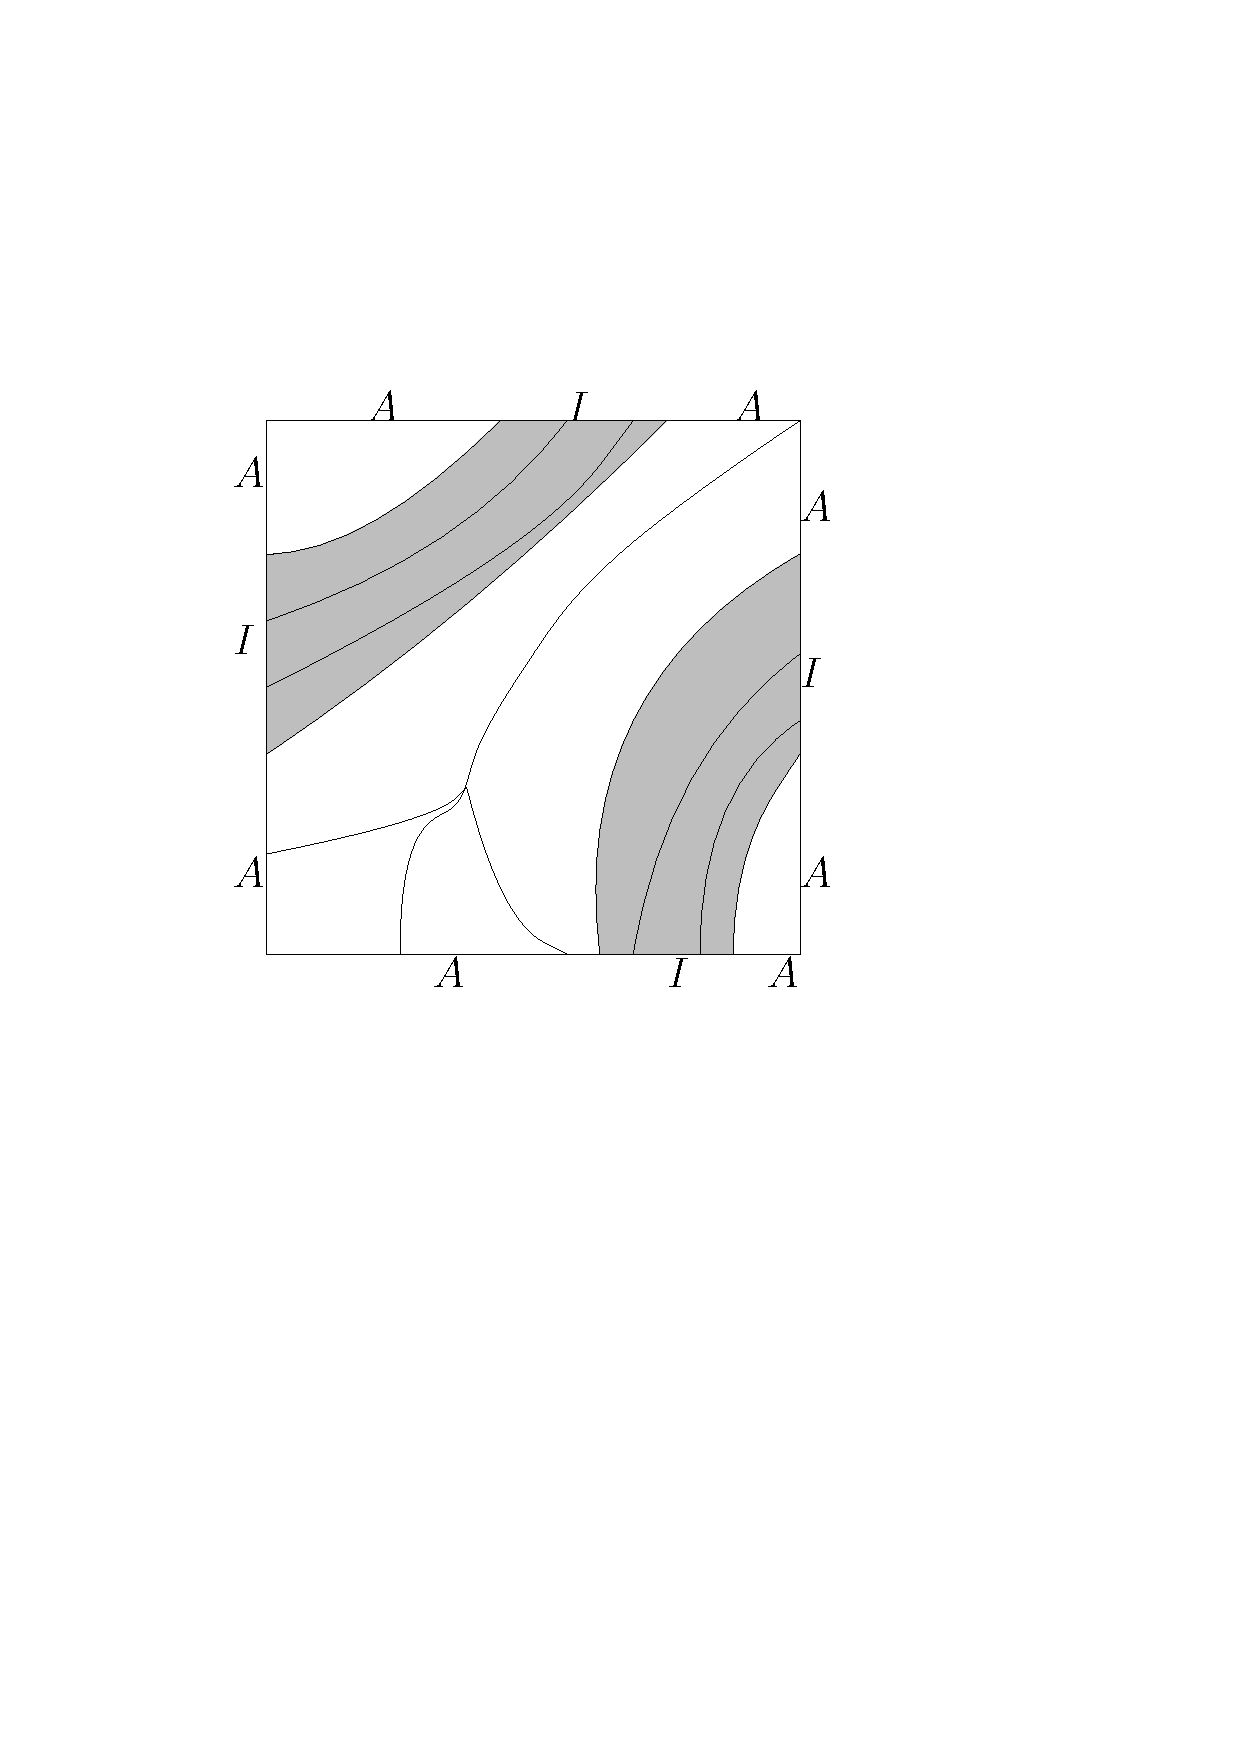
\includegraphics[width=0.5\textwidth]{figures/activeinactiveregions.pdf}
	\caption{Here the white regions are active and the shaded regions are inactive. The 
    		 boundaries between the regions encapsulating active and inactive region, are 
             defined by being the bisector of one marked and one unmarked generator.}
	\label{fig:activeinactiveregions}
\end{figure}

The algorithm will compute the active regions, which can be done in a time that is proportional to the 
number of marked generators in the cell $c$. Overall can this be done since we know the order of the 
generator along the boundary of $c$, which will help us finding the marked generators with unmarked 
neighboring generators. The calculated boundary of these active regions will have $O(1)$ segments. 
These segments will either be a transparent edge fragment, an opaque edge, of a bisector in $SPM(s)$.

We now let $e$ be a transparent edge fragment that's bounding an active region. Further let $W(e)$ be 
the wavefront that enter the active region by crossing edge $e$. Should $W(e)$ be the only wavefront 
entering through $e$, it will partition the active region into piece which we call $S$-faces. Each 
$S$-face has a unique predecessor in the $W(e)$ partitioning the area. The $S$ faces of an active 
region may not cover all of it, since each point in an $S$-face must be connected to its predecessor 
by a segment that intersect $e$. We define $S(e)$ to be this partition. So basically $S(e)$ are the 
building blocks of a shortest path map, which restricts the active regions and considers only 
generators in $W(e)$. Let assume a point $p$ lies in an $S$-face of $S(e)$ with predecessor $v$, then 
$S(e)$ assigns weight $d(s,v) + |\overline{vp}|$ to $p$. Points outside any $S$-face are assigned 
infinite weight by $S(e)$.

We can compute $S(e)$ in $O(m\log m)$ time, where $m = |W(e)|$, by using the propagation algorithm and 
the auxiliary data structures which will be introduced in section \ref{section:implwavefront}.

\subsubsection{Proof of correctness for computation of SPM}

The following proofs are taken from \cite{HershbergerS99}, and included for completeness.

The following lemma shows how to combine the wavefronts incident to different
boundary edges of an active region.

\begin{Lemma}[Lemma 4.12 in \cite{HershbergerS99}] \label{lemma:4.12} 
	Given the approximate wavefronts on the boundary of a cell $c$ and a set of
	$k$ marked generators in those wavefronts, we can compute the vertices of
	$SPM(s)$ inside $c$ in time $O(k\log k)$.
\end{Lemma}
\begin{proof}
	Consider an active region inside $c$ and two transparent edge fragments $e$
	and $f$ on the boundary of this active region. We can use the merge step
	from a standard divide-and-conquer Voronoi diagram algorithm to compute the
	portion of the region nearer to $W(e)$ than to $W(f)$ using weighted
	distance in time $O(|W(e)|+|W(f)|)$. More specifically assume that $S(e)$
	and $S(f)$ have both been computed. Let $m=|W(e)|+|W(f)$. Each of $S(e)$
	defines a distance function on the points of the active region. The
	pointwise minimum of these two functions determines which points are nearer
	to $W(e)$ than to $W(f)$ under weighted distance. Consider a point $p$ in
	the $S$-face for some generator $v\in W(e)$. Point $p$ belongs to $v$'s
	$S$-face in $SPM(s)$ only if all of the segment $\overline{pv}$ is closer to
	$v$ than to any generator in $|W(f)|$. The set of  points $p$ such that the
	entire segment from $p$ to its predecessor is closer to $W(e)$ than to
	$W(f)$ is bounded by a single chain $\Gamma$ of $O(m)$ hyperbolic arcs. (The
	number of arcs follows from Lemma \ref{lemma:3.2}.) To find $\Gamma$, first trace along
	a ray emanating from some generator $v \in W(e)$ marching through $S(e)$ and
	$S(f)$ simultaneously until the ray reaches the boundary of $c$ or reaches a
	point whose weight in $S(f)$ equals its weight in $S(e)$. This takes $O(m)$
	times since a line cuts $O(m)$ edges of $S(e)$ and $S(f)$ containing the
	current point trace along the hyperbola until it leaves one of the two
	$S$-faces then follow the hyperbola determined by the next pair of $S$-faces
	etc. This procedure takes $O(1)$ time per arc of $\Gamma$ or $O(m)$ time
	altogether (see Figure \ref{fig:traceray}). 
    
\begin{figure}[H]
	\centering
	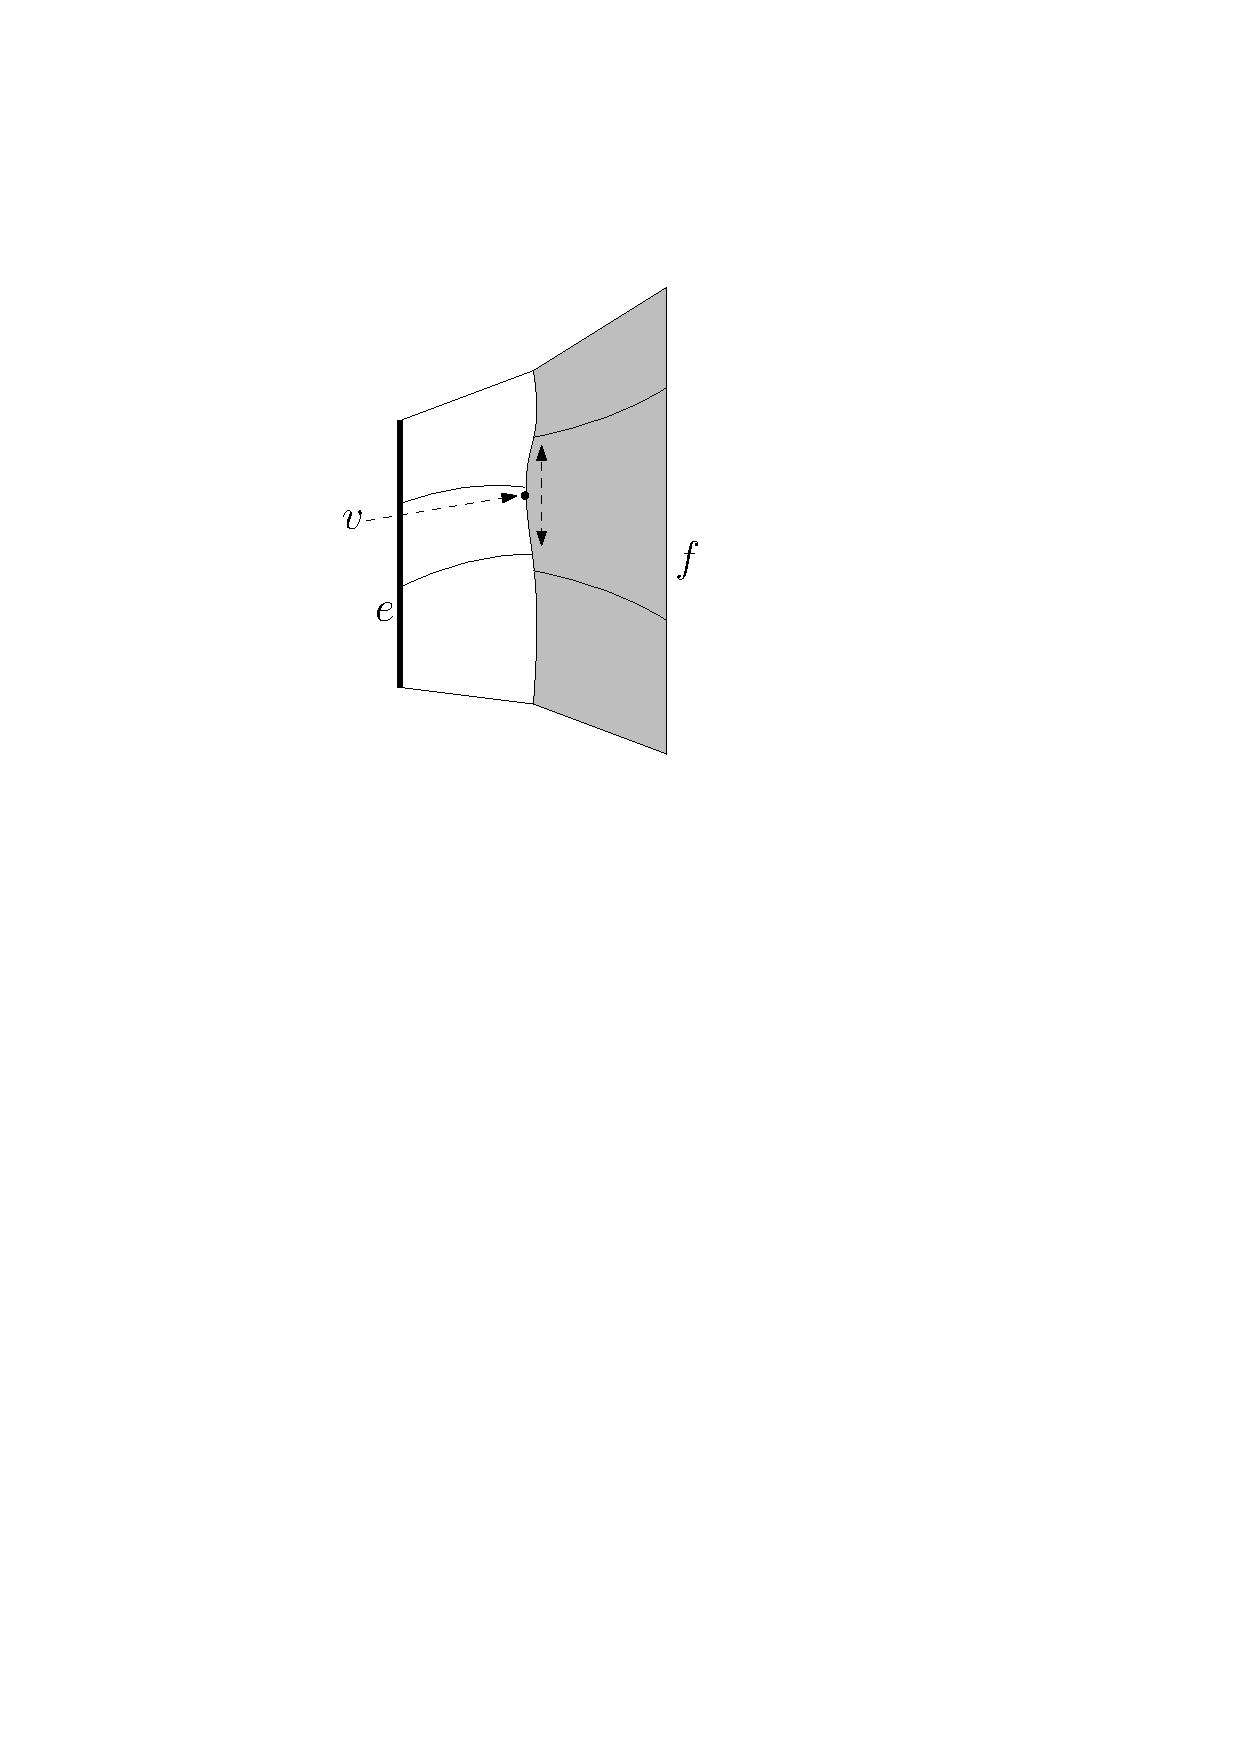
\includegraphics[width=0.35\textwidth]{figures/traceray.pdf}
	\caption{To find the region close to $W(e)$ than to $W(f)$ under weighted distance, 
    		 trace a ray from some $v \in W(e)$ through $S(e)$ and $S(f)$ until it hits a point 
             equidistant from the two wavefronts, then trace outward from the point along the bisector 
             $\Gamma$}
	\label{fig:traceray}
\end{figure}
    
    The tracing procedure computes region closer to
	$W(e)$ than to $W(f)$ for one edge $f$. Intersecting the results for all
	such edges $f$ on the boundary of the active region produces the region
	$R(e)$ claimed by $W(e)$ in $SPM(s)$. Intersecting $R(e)$ with $S(e)$ gives
	vertices of $SPM(s)$ to which $W(e)$ contributes. We repeat this computation
	for each transparent edge fragment to find all the vertices of $SPM(s)$ in
	%side 26
	the active region. Applying this algorithm to all active regions finds all
	vertices of $SPM(s)$ inside $c$.

	The partition $S(e)$ determined by each edge fragment $e$ participates $O(1)$
	times in a Voronoi-style merge, so the total cost of merging is $O(k)$.
	Hence the running time is dominated by the propagation algorithm which takes
	$O(k\log k)$ times altogether.
\end{proof}
\begin{Lemma}[Lemma 4.13 in \cite{HershbergerS99}] \label{lemma:4.13} 
	The shortest path map vertices computed cell-by-cell can be combined to
	build $SPM(s)$ in additional $O(n\log n)$	 time.
\end{Lemma}
\begin{proof}
	To compute $SPM(s)$ we compute all its edges separately then use a standard
	plane sweep to assemble them as follows. Create a list of the bisector
	endpoints discovered in the computation of Lemma \ref{lemma:4.12} each identified by a
	key consisting of two generators. Put each three-bisector endpoint into the
	list three times, once for each bisector. Put each bisector/edge collision
	in once labeled with the generators of the bisector. Now sort the list to
	group together endpoints belonging to each bisector. Take the endpoints
	belonging to the bisector of a generator pair $(v,w)$ and sort them along
	the hyperbola determined by the weighted generators of $v$ and $w$. This
	determines all edges of $SPM(s)$ on the hyperbola. Doing this for all pairs
	that appear as keys in the sorted list gives all $O(n)$ hyperbolic arcs of
	$SPM(s)$. Finally with a standard plane sweep, we can combine these arcs
	with the edges of $\mathcal{O}$ to build the subdivision $SPM(s)$.
\end{proof}

\section{The list based data structure for wavefront propagation} \label{section:datastructurewavefront}

To keep track of our approximate wavefront, we use a list to keep track of the generators coming from 
obstacle vertices. For this list we need a data structure which we can use two types of operations on:

\begin{enumerate}
\item \textit{Standard list operations:} these are insert, delete, concatenate, split, find previous 
			  and next element, and search. Here the search operation locates the position of a query 
              point. This position is found in the list of bisectors defined by the generators 
              wavefront at a particular time. 
\item \textit{Priority queue operations:} this operations are used on the generators, to which we 
			  assign a priority. The data structure should be able to  update priorities and find the 
              minimum priority in the list.
\end{enumerate}

These two types of operations should be implemented in a flavor of self balancing binary trees. One 
could implement the operations e.g. in a red-black tree. Here the generators will be located at the 
leaves, and each node should have a priority field which records the minimum priority of the leaves in 
it subtree.

The only requirements to the flavor of self balancing binary tree is the list operations should each 
take $O(\log n)$ time to process on a list of length $O(n)$. Each priority operation should likewise 
take $O(\log n)$ time each. 

Beside these operations we also need the tree to be fully persistent, s.t. we can operate on past 
version of any list. Each kind of operation uses $O(1)$ storage per node of the binary tree, which 
mean we can make the data structure fully persistent by path copying. The effect of using an operation 
affects $O(\log n)$ nodes of the tree, which also includes the ancestors of every affected node. We we 
simple, before an operation modifies the tree, we copy all the nodes that will be affected, and then '
modify the copies. This way we create a new version of three while leaving the old version unchanged.
Since the data structure uses $O(\log n)$ for each operation, and we save a copy of size $O(\log n)$, 
the total storage usage of the data structure is $O(m \log m)$ where $m$ is total number of operations 
used. The above gives us the following lemma:

\begin{Lemma} [Lemma 5.1 in \cite{HershbergerS99}]
There is a linear-space data structure that represents an approximate wavefront an supports list 
operations and priority queue operations in $O(\log n)$ time per operation. The data structure can be 
made fully persistent at the expense of an additional $O(\log n)$ space per operation.
\end{Lemma}

\section{An implementation of the wavefront propagation} \label{section:implwavefront}

Concretely the idea of wavefront propagation is to propagate an approximate wavefront from an edge edge on 
the boundary of the cell containing the edge we want to propagate to. In particular, we want to propagate 
the wavefront $W(e)$, an compute $W(e,g)$ for ever edge $g \in output(e)$, and in this process, assign the 
time (weight) of first contact between $W(e,g)$ and the endpoints of $g$.In this section we will show how 
to do this computation of $W(e,g)$ for all transparent edges $g$ on the boundary of $e$'s cell. 

We know from lemma \ref{lemma:4.1} that there is a constant number of edges in $output(e)$, which means 
they can only belongs to a constant number of different cell. We will use this fact to compute $W(e,g)$ 
for all $g \in output(e)$. When propagating the wavefront cell-by-cell, we can think of this as splitting 
the wavefront $W(e,g)$ into multiple piece, each piece is labeled by the sequence of crossings of 
transparent edges it follows from $e$ to $g$. The $W(e,g)$ is then made of these components wavefronts by 
concatenating the piece that are topological equivalent paths inside $\mathcal{U}(e)$. 

Since each of these component wavefronts is a list of generators, we may find that adjacent wavefront 
piece can contain duplicate generator that claims the common endpoint. On of these duplicates are to be 
deleted before the lists are concatenated.

As an example of the above see figure \ref{fig:weg}. Here $W(e,g)$ is assembled from $W(e',g)$ and 
$W(e'',g)$, where $e'$ and $e''$ are two edges on the boundary of $g$'s cell.

\begin{figure}[H]
	\centering
	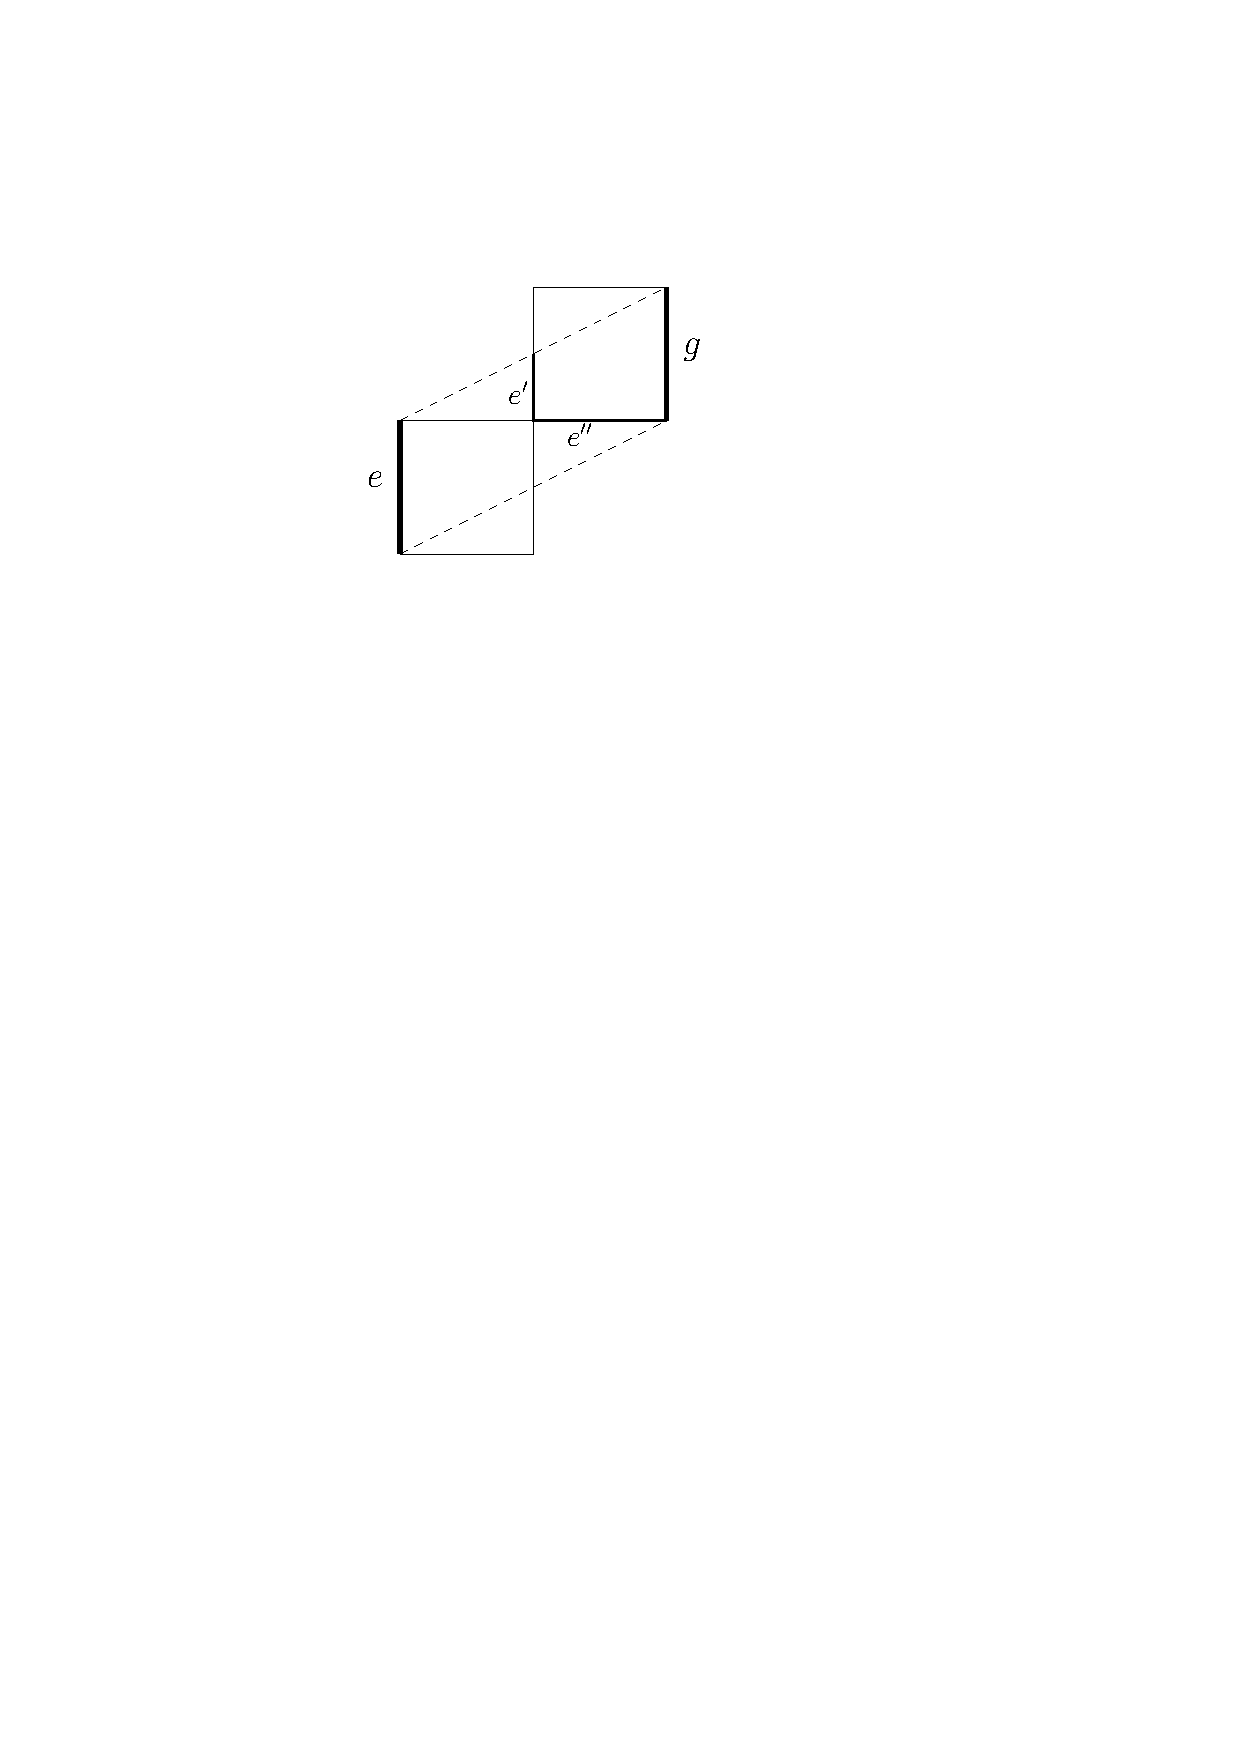
\includegraphics[width=0.4\textwidth]{figures/weg.pdf}
	\caption{$W(e,g)$ is assembled from $W(e',g)$ and $W(e'',g)$, where $e'$ and $e''$ are two edges on 
    		 the boundary of $g$'s cell}
	\label{fig:weg}
\end{figure}

The propagation algorithm which follows assumes that each cell $c$ is convex. Since we assumed the 
conforming subdivision could be build with square annulus, this isn't satisfied immediately. For this we 
temporarily break a cell which isn't convex into subcells by adding transparent edges, which are 
\textit{parallel to $e$} through the points of nonconvexity. An example of this i shown in figure 
\ref{fig:preparingcells}.

\begin{figure}[H]
	\centering
	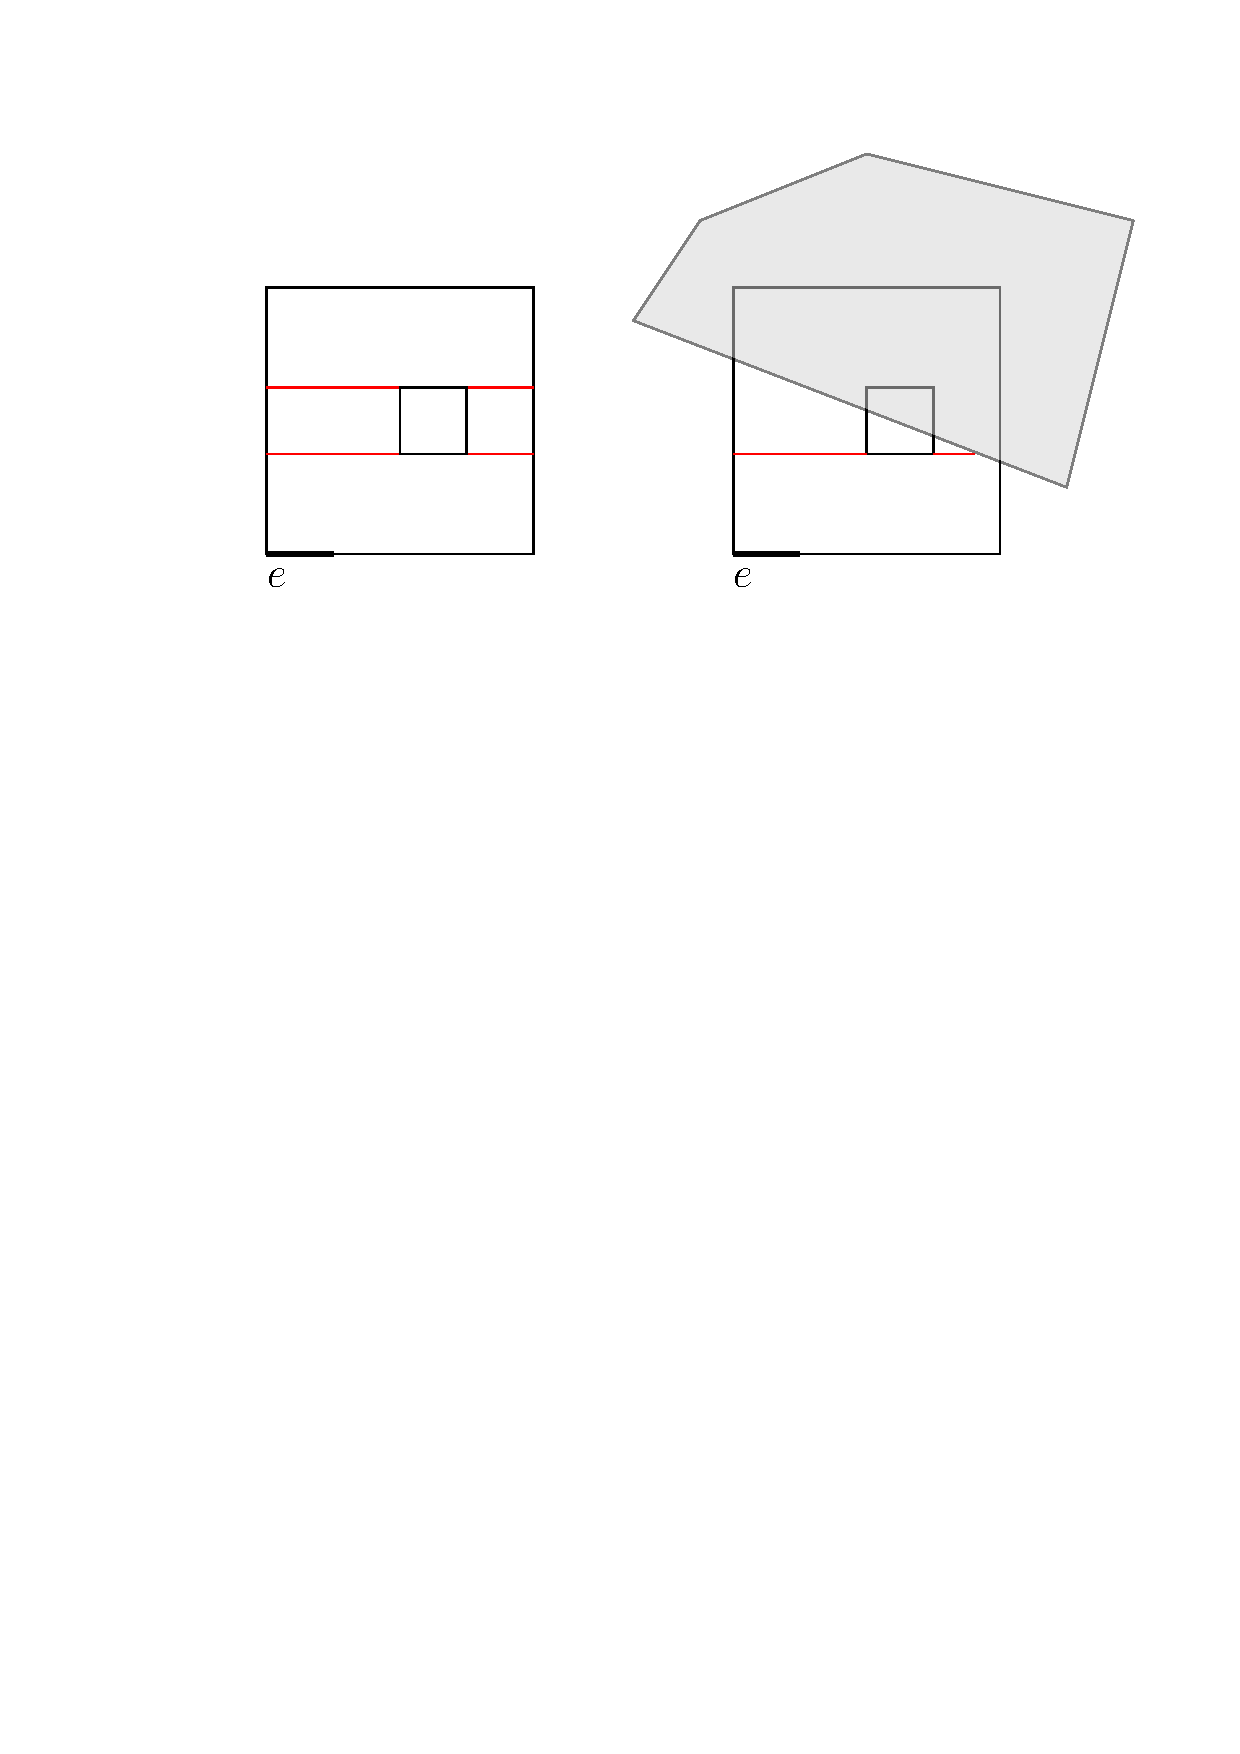
\includegraphics[width=0.7\textwidth]{figures/preparingcells.pdf}
	\caption{Insertion of transparent edges parallel to $e$ to fix the cells non convexity. The right 
    		 figure is the cases of an obstacle overlaying the cell.}
	\label{fig:preparingcells}
\end{figure}

Let $f$ a transparent edge of the boundary of $c$ such that $f \neq e$. Then the propagation algorithm has 
the following invariant.

\paragraph{Propagation Invariant:} When a wavefront $W(e,f)$ is propagated for distance $2 \cdot | f |$
           beyond $f$, it intersects only a constant number of cells of the conforming subdivision 
           of the free space.  \\

We already saw in the former chapter that the conforming subdivision $S'$ already satisfy the Propagation 
Invariant, since, by the propagation invariant, each edge $f$ is well-covered with parameter 2. But since we 
just added some temporary transparent edges to non convex cells, we need to fix these in a way that abides to 
this invariant. This is done by dividing these added edges into $O(1)$ pieces, each no longer than the edges 
of $\mathcal{S}$ on the boundary of the annulus's outer boundary, one-eight the side length of the outer 
square, which we know is bounded by the minimum clearance property and uniform edge property of the conforming 
subdivision, see section \ref{section:def-well-covering-if-regions}. 

We know let $H$ denote the convex hull of $e$ and the inner square of the annulus as shown in figure 
\ref{fig:subdividedconvexhull}. Should $H$ intersect an added transparent edge $f$, we further subdivide the 
sub edge $f \cap H$ into pieces of length equal to the inner square of the annulus, as also shown on figure 
\ref{fig:subdividedconvexhull}. 

\begin{figure}[H]
	\centering
	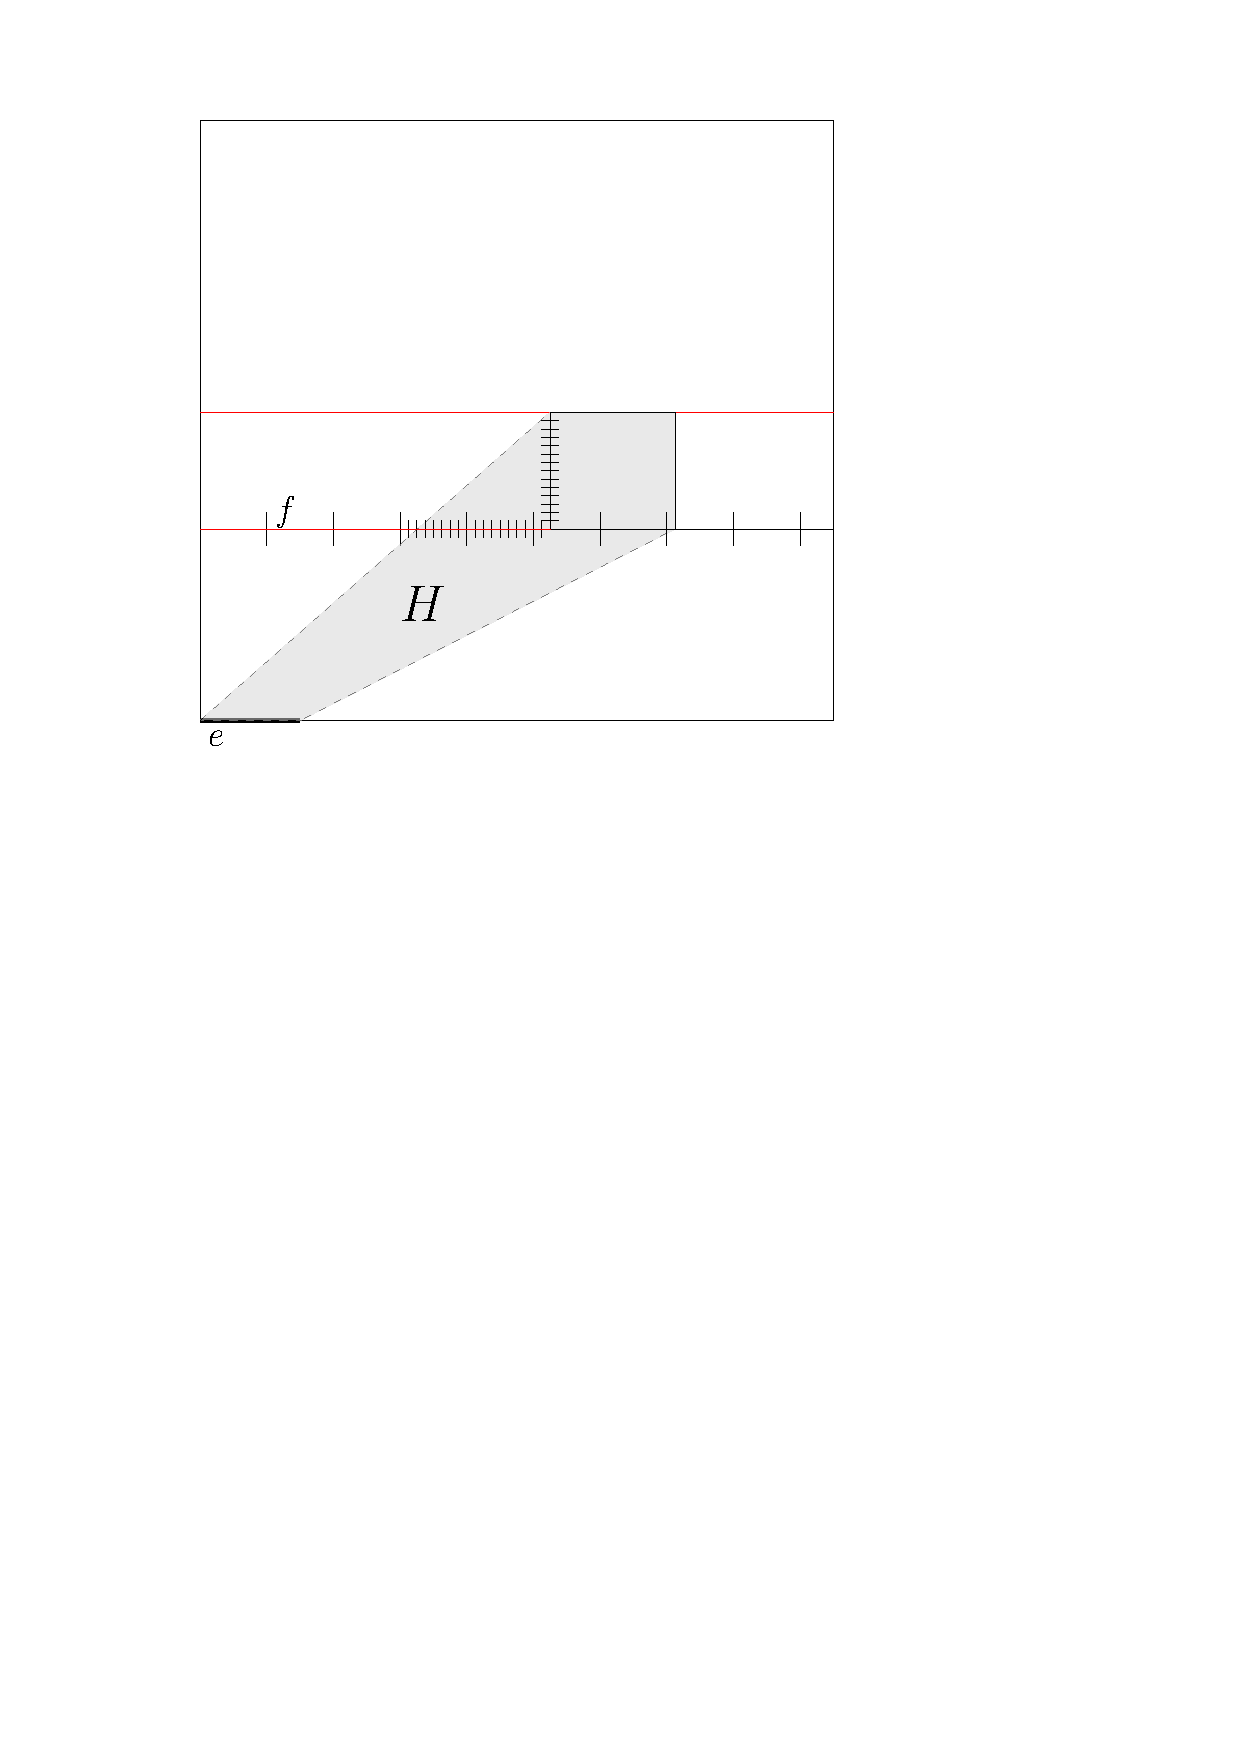
\includegraphics[width=0.6\textwidth]{figures/subdividedconvexhull.pdf}
	\caption{A subdivision of of a cell, with a convex hull around a boundary edge $e$ and the inner square of 
    		 the annulus.}
	\label{fig:subdividedconvexhull}
\end{figure}

Due to $f$ being parallel with edge $e$ and the inner boundary of the annulus being well separated from the '
outer boundary, see again the minimum clearance property, the total length of $f$'s sub edge inside $H$ is 
proportional to the side length of the inner square. By this it follows that the partition of $f$ only creates 
$O(1)$ edges. We can see that these subdivided edges satisfy the propagation invariant, by the following example. 
Given any such $f$, let $g'$ be an edge of $c$ such $W(e,f)$ leaves $c$ by passing through $g'$. Since $g'$ is an 
edge from the conforming subdivision of the free space, $\mathcal{S}'$, we know it is a fragment of an edge $g$ in 
the conforming subdivision of the obstacles vertices and $s$, $\mathcal{S}$. We know we from lemma 
\ref{lemma:admitsa2conformingsubdivision} that there are $O(1)$ cells of $S'$ within shortest path distance $2|g|$ 
of $g'$ by construction. Since the new transparent edge which makes the cell $c$ convex are subdivided into piece 
such that $|f| \leq |g|$, then this implies that the propagation invariant holds for the edge $f$.

\subsection{Dynamic wavefront propagation} \label{section:dynamicwavefront}

Up until now we have, in this chapter, kept the simulation of wavefront propagation rather static, in the sense that
we have look at the atomic examples of how to handle different cases at different time in the propagation process.
Now we take these ideas and see what happens when we let them operate in a dynamic setting. This means e.g. 
since a wavefront is a collection of generators, which one of the generators waves do we calculate first, and how do
we drop a generator when it has served its purpose, and so on. So we see what happens to the wavefront propagation 
when we add the element of time to the process.

So what happens to the combinatorical structure of the wavefront as it sweeps across the (convex) cells, and how 
does the wavefront $W(e)$ behave as it sweeps across a cell $c$ after entering it through the edge $e$? The 
simulation should detect and process each bisector event involving the the generators from each wavefront, e.g. 
$W(e)$ that may occur inside $c$. The events are processed in an order of increasing distance to $s$. This is to 
simulate the element of time since the weight and therefore the distance to each generator is assigned by the 
arrival of the wavefront in unit speed, so distance and time are equivalent in this sense. So generator marked as 
event are process.

Let $W$ denote the current wavefront we currently are simulating, at any time in its simulation process. In the 
beginning of the simulation we have $W = W(e)$ as the approximate wavefront which passes through $e$ to compute cell
$c$. It might be the case that the edge $e$ is claimed by multiple waves, and therefore $W$ is a list of generators,
each claiming a portion of $e$. Every generator $v \in W$ defines a pair of bisectors with its neighbors in the 
list. If we let $v$ be the first generator in the list, then $v$ claims one of the endpoints of $e$, and its first 
bisector represented as the ray from $v$ through the end point of $e$. Similarly we define the last generator $v'$ 
of the generators. Should $v = v'$ and claim the whole edge $e$, then there are no bisectors in the list, and the 
wave is the ray propagated from the generator through $e$. See figure \ref{fig:vandvprimesharingedge}, \ref{fig:vandvprimeallofe} and \ref{fig:visallofe}.

\begin{figure}[H]
	\caption{Crossing of two line segments}
	\minipage{0.48\textwidth}
		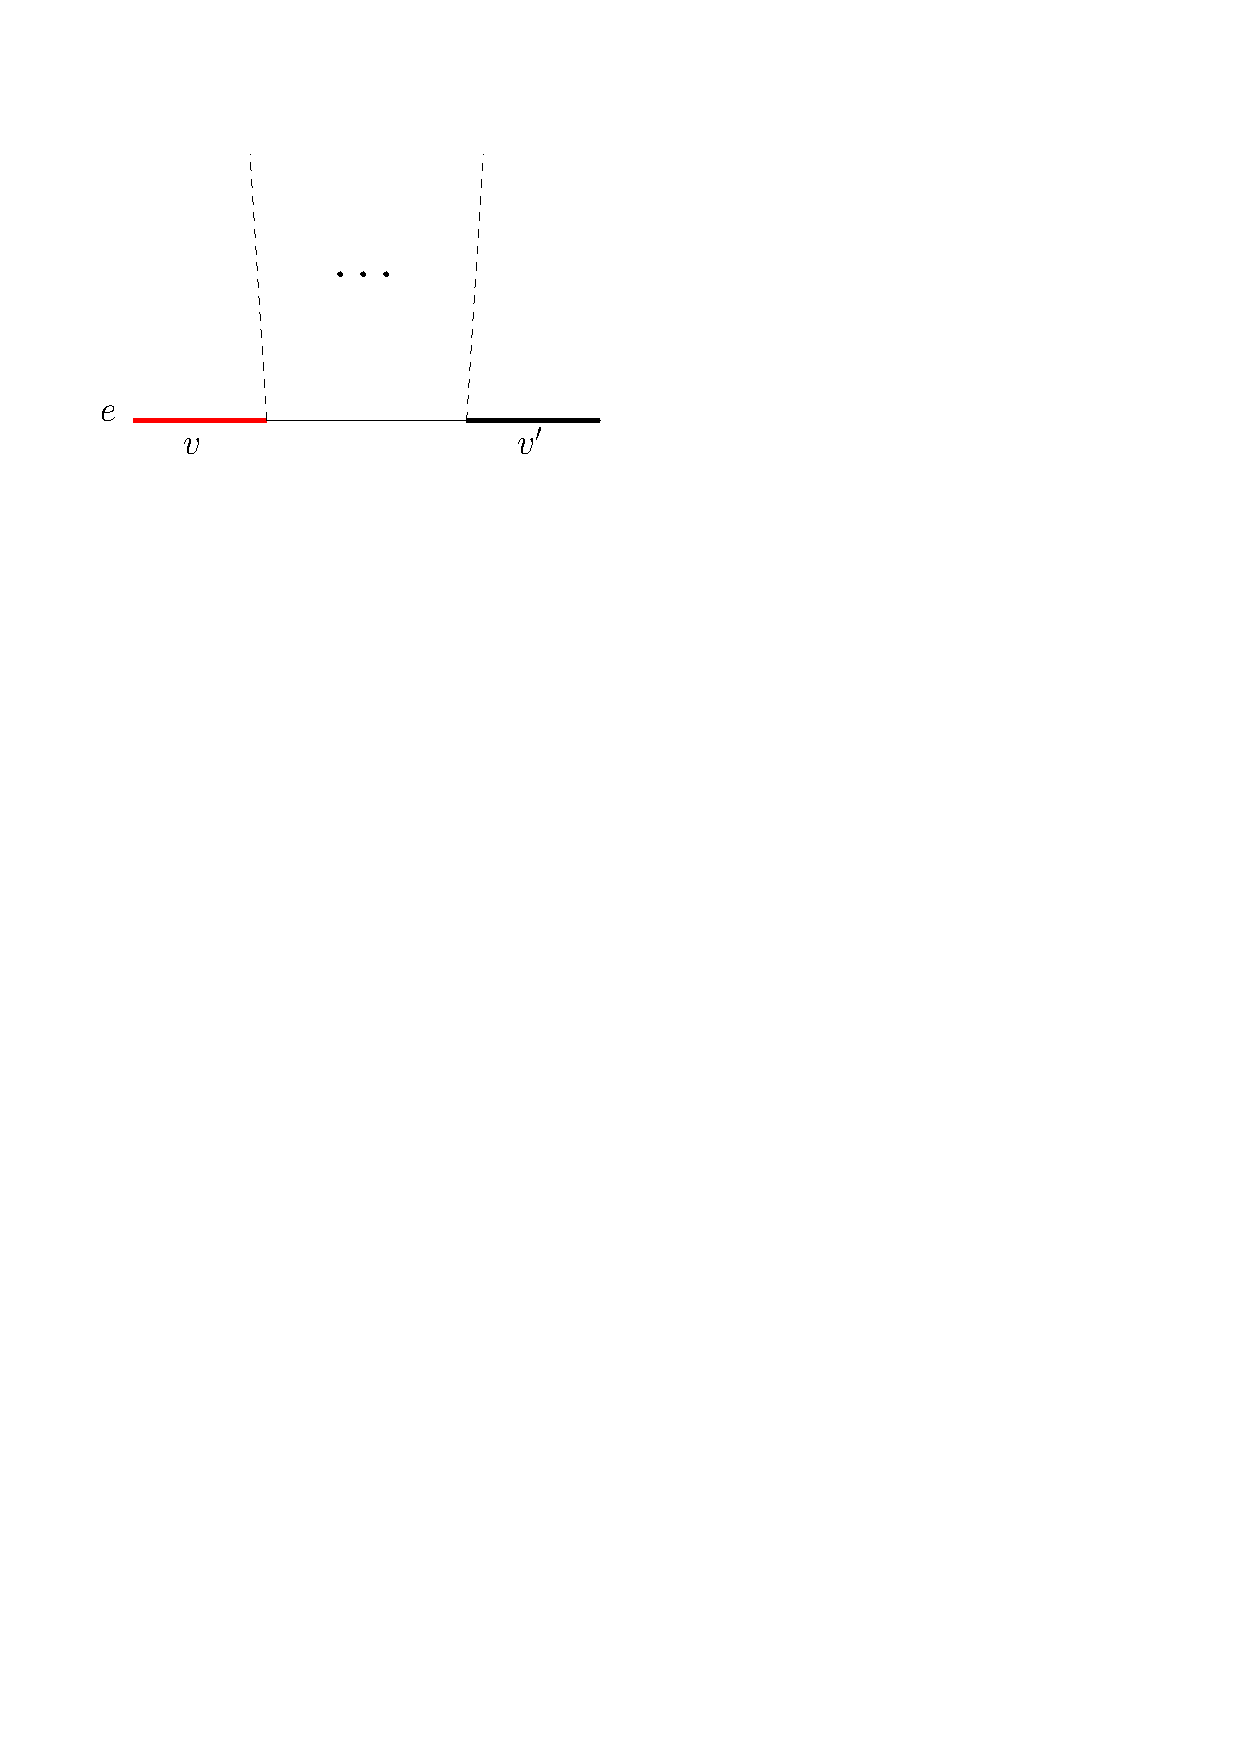
\includegraphics[height=3cm]{figures/vandvprimesharingedge.pdf}
		\caption{$v$ and $v'$ each claim the end points of $e$, with their bisectors being shared with other generators claiming the middle part of $e$.}
		\label{fig:vandvprimesharingedge}
	\endminipage\hfill
	\minipage{0.48\textwidth}
		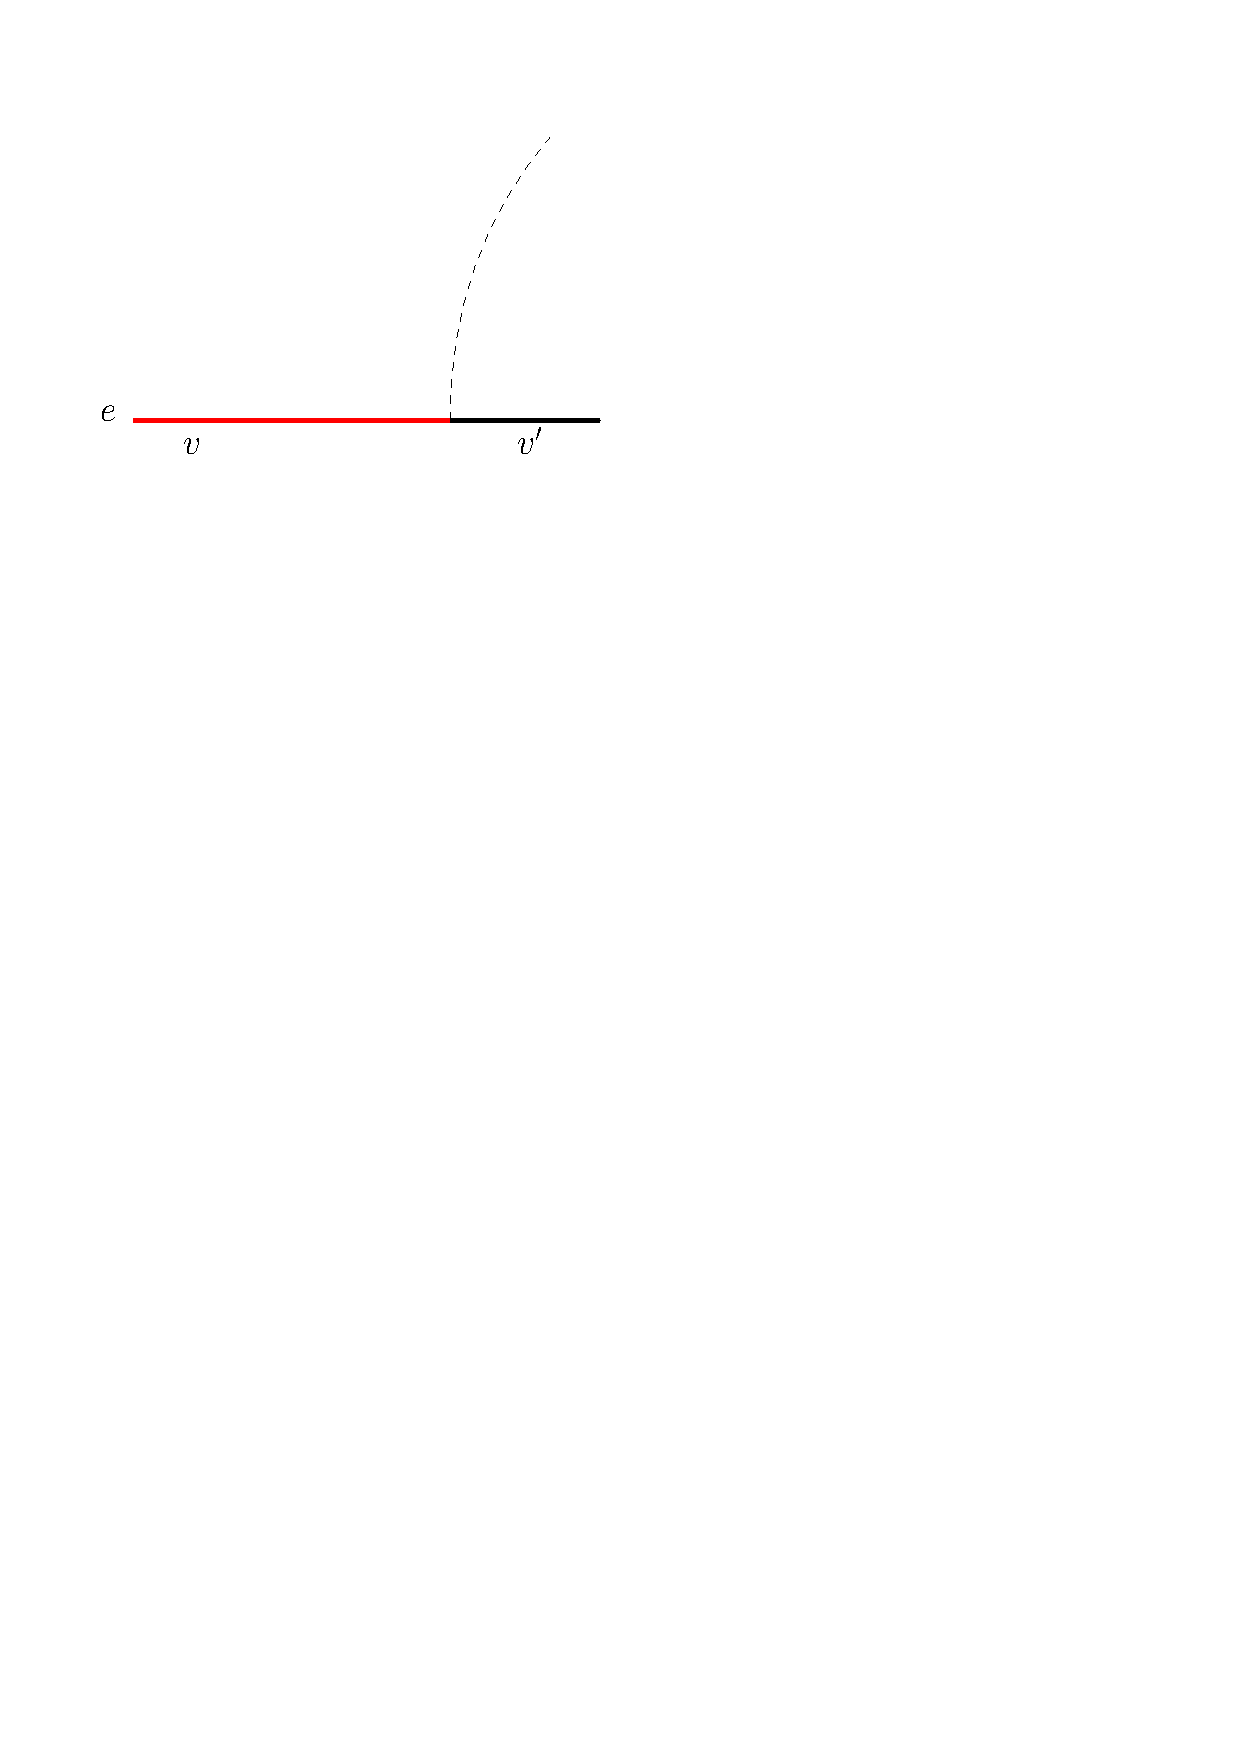
\includegraphics[height=3cm]{figures/vandvprimeallofe.pdf}
		\caption{$v$ and $v'$ claim all of $e$ and only have one bisector between them}
		\label{fig:vandvprimeallofe}
	\endminipage\hfill
	\centering
	\minipage{0.5\textwidth}
		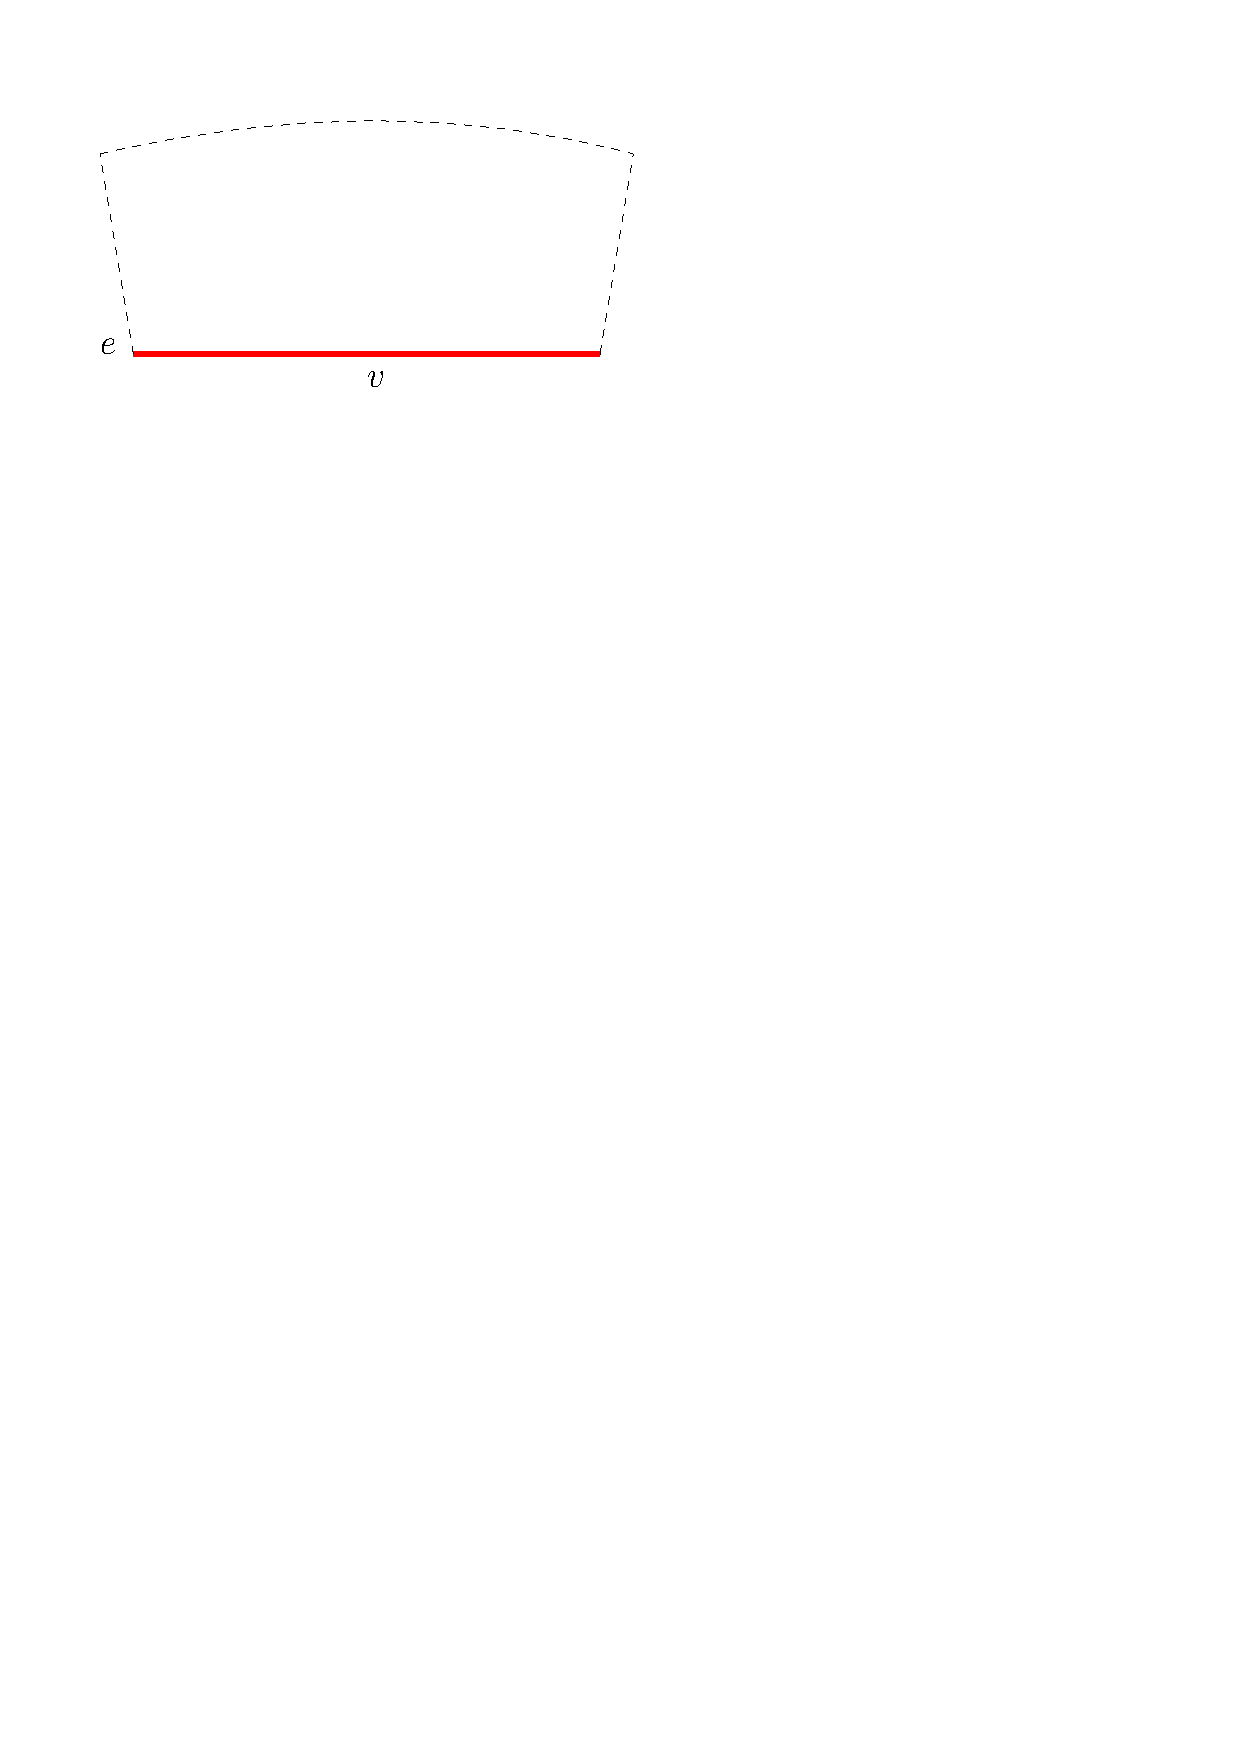
\includegraphics[height=3cm]{figures/visallofe.pdf}
		\caption{$v$ claims all of $e$ and there are therefore no bisectors other than the ray projected from $v$ through $e$.}
		\label{fig:visallofe}
		\endminipage\hfill
\end{figure}

In order to process the bisectors event in the correct order, we will maintain the generators of $W$ in the priority queue which was 
describe in section \ref{section:datastructurewavefront}. The priority field which each node of the priority queue tree has, is 
assigned with its weighted distance to the point at which the two bisectors that defines $v$ and its neighbors intersect, beyond $e$. 
An example of this is given in figure \ref{fig:priorityvalue}. Here thee bisectors defining $v$ and its neighbours intersects after 
passing through $e$, and meeting at the point $p$. This means that $v$ priority value $priority(v) = d(s,v) + |\overline{vp}|$.

\begin{figure}[H]
	\centering
	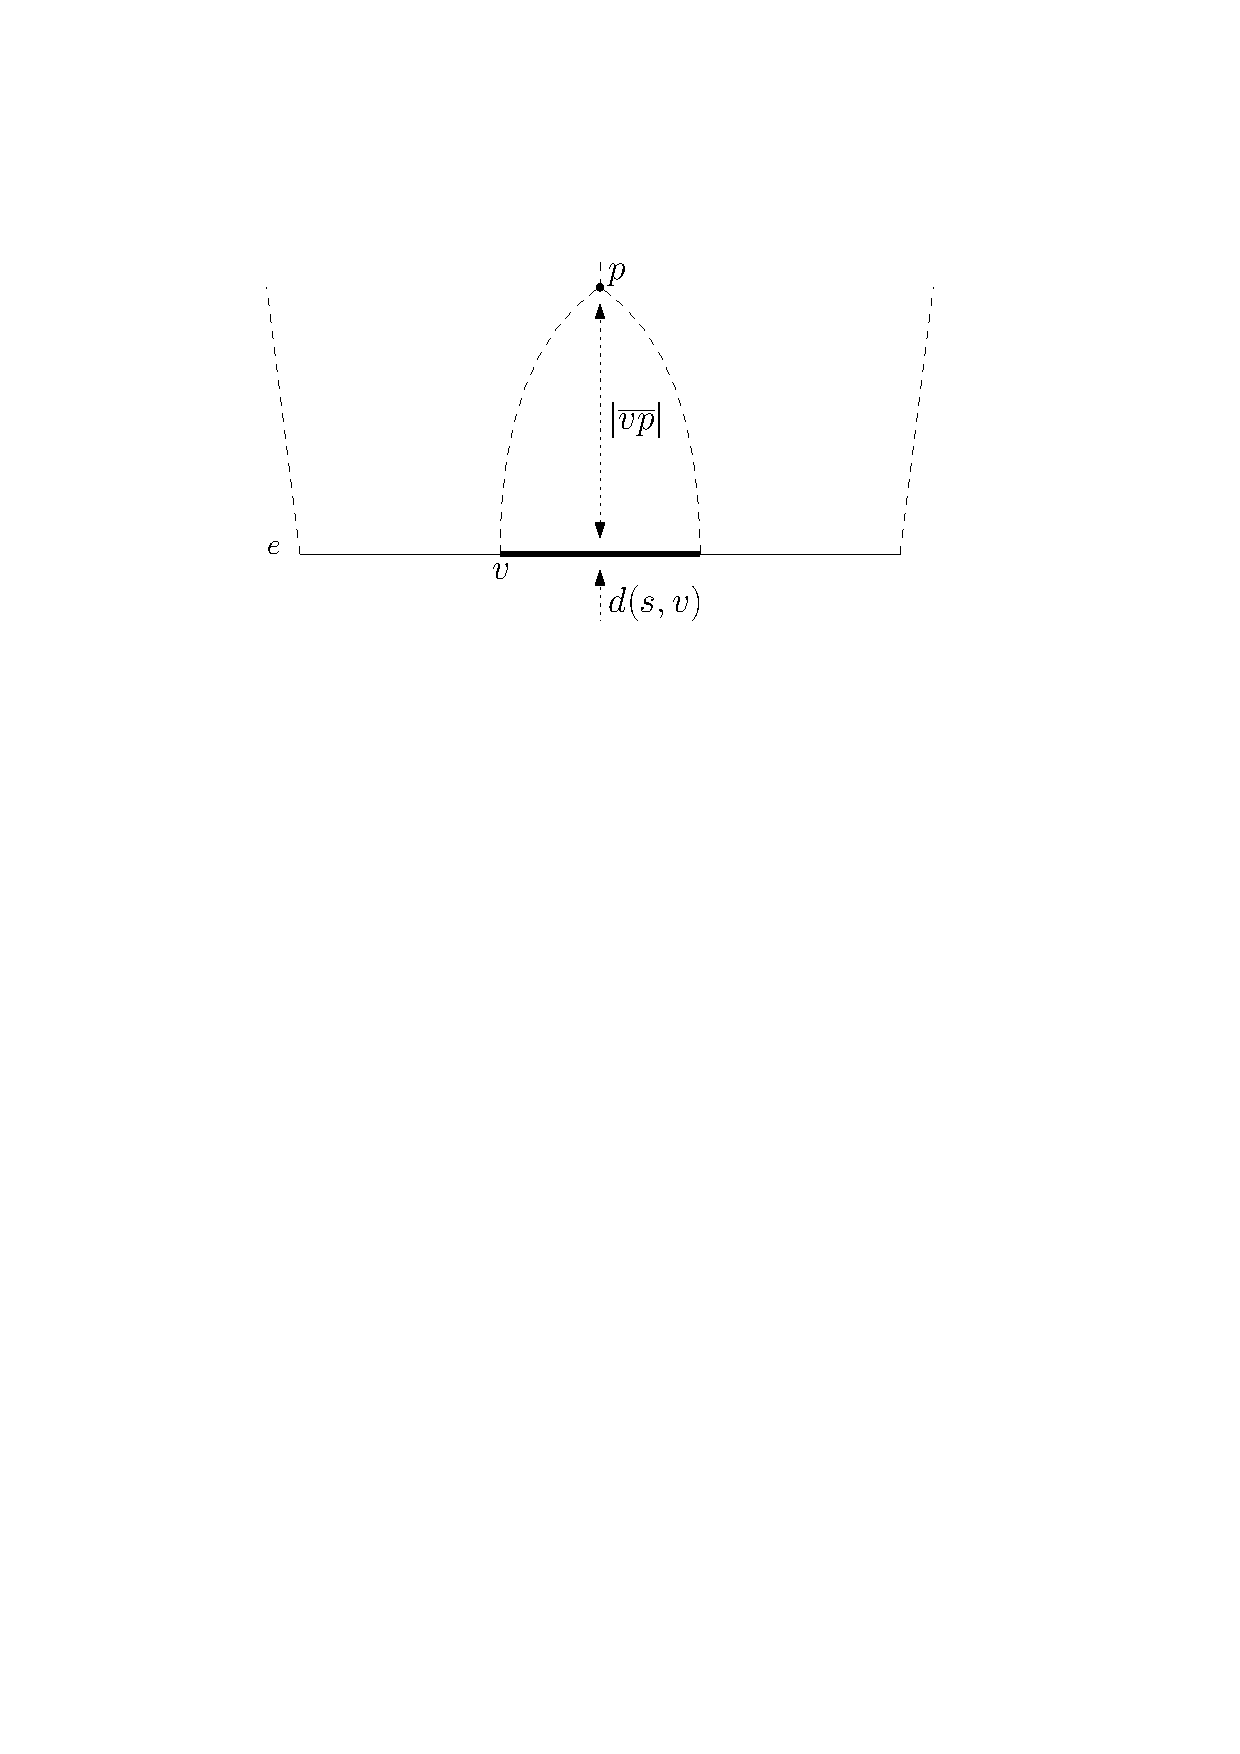
\includegraphics[width=0.8\textwidth]{figures/priorityvalue.pdf}
	\caption{A visualization of what a generator $v$'s priority value, $|\overline{vp}| + d(s,v)$, could be with the
	         dashed lines being bisectors of the generators claiming $e$.}
	\label{fig:priorityvalue}
\end{figure}

The processing of the approximate wavefront propagation will be done in event of increasing priority up to some maximum priority 
$t_{stop}$. The $t_{stop}$ is calculated from the shape of the cell $c$, which we will show how to later in this section. The limit of 
$t_{stop}$ is calculated from the individual values of $t_{stop}(f)$ for each transparent edge $f$ of $c$. Initially the values for all
f is $t_{stop}(f) = \infty$ and therefore $t_{stop} = \infty$. Also to keep track of the priorities through out the simulation, by 
initializing an empty set $T$ which will be cleared after each simulation.

At each step of the simulation, the generator $v$ with the lowest priority from the queue is processed, where one of following 
scenarios can happen.

\begin{enumerate}
    \item  If the event (the intersection of the $v$'s bisectors) happens inside the cell $c$, then $v$ is deleted, since it no longer 
           propagates the free space, and we recompute the priorities for $v$'s neighbours. We mark $v$ in $W(e)$ for the cell $c$ by 
           the marking rules explained in section \ref{section:bisectorevents}, which also implies marking it in $O(1)$ number of 
           neighbouring cells to $c$ accord to the marking rules.
    \item If $v$'s event happens outside, then we set $priority(v) = \infty$ and add $v$ to the set $T$. In this case the generator 
          list is not changed since $v$ still has more free space outside of $c$ to propagate.
\end{enumerate}

If we where to process each bisector event of $W$ in their initialize time order, and not update them in the first of the above cases, 
then the neighboring generators of $v$ could participate in bisector event outside of cell $c$ before, all bisector events inside $c$ 
were fully processed. 

So far we have seen the intersection of $v$'s bisectors if its neighbours engulfs $v$, as seen in figure \ref{fig:priorityvalue}, in 
which case we would mark $v$ by rule 3 of the generator marking rules. But it's also important to be aware that the bisector event of 
$v$ could also happen if either the intersection lies on a opaque edge of if they lie on different transparent edges with an opaque 
edge between them. In that case rule 1 above, should still do as stated, but would use rule 4 to mark $v$ for cell $c$ and its 
neighbours. Should the intersection point $p$ lie on a transparent edge, e.g. $f$, then we update our $t_stop$'s as follows:

\begin{align*}
    t_{stop}(f) &= \min(t_{stop}(f), d(s,v) + |\overline{vx}| + |f|) \\
    t_{stop}    &= \min(t_{stop}, t_{stop}(f))
\end{align*}

The update of $t_{stop}(f)$ is either the current $t_{stop}(f)$ or the weight as calculated the same way as in figure 
\ref{fig:priorityvalue} plus the length of the transparent edge $f$. This way we assure, that overestimate the priority since we would 
have swept all of $f$. By doing it this way, we also don't overshoot the estimate since it still not $2\cdot|f|$ times greater than the
time at which $W$ first comes to contact with $f$.

The $t_{stop}$ priority, which is in the priority queue, is either $t_{stop} = \infty$ in which case all events inside $c$ have been 
processed, or $t_{stop} < \infty$, which happens in the above update if there is a transparent edge $f$ on the boundary of $c$ with 
$t_{stop} = t_{stop}(f)$. We see that by updating $t_{stop}(f)$ this way, we ensure that all bisector events needed to produce $W(e,f)$
have indeed been processed. So now we move one to explain how to process $W(e,f)$. The wavefront $W(e,f)$ is calculated from $W$ in the
following way. First we locate the endpoints of $f$ in $W$, which can be done by can picking a bisector in $W$, and following its 
neighbors outwards, there is at least on such bisector (in the case of one, this bisector claims all of f). Mark the endpoint claiming 
generator by rule 2. From here we split the generator list into 3 parts. Those generators whose bisectors are between the two endpoint 
claiming generators. Those are the one who will go through $f$, which after the reset of priorities will be the $W(e,f)$ wavefront, and
the other two sets are those who pass left and those who pass right of $f$. The simulation process continues with the left and right 
passing sets independently after the $t_{stop}$ has been reset in each set to be the minim of $t_{stop}(g)$ over the transparent edges 
$g$ for that group. 

\missingfigure[]{}

So the above is the case of $t_{stop} < \infty$. Should we stop because we reach $t_{stop}$ and $t_{stop} = \infty$ then we split the 
current generator list at all the transparent edge endpoints, which will produce $W(e,f)$ for each transparent edge $f$, and some 
wavefront pieces that hit only opaque edges.

Should no transparent edges remain in some piece, then all bisectors in the piece hits an opaque edge, in which case we mark all the 
generators in that piece for cell $c$ and a $O(1)$ of neighboring cell by marking rule 4. We also make the necessary marking of rule 2 
and rule 3.

When finished the priority of each vertex in $T$ is reset, based on the bisectors it defines with its neighbours in the new list. This 
is done to ensure each wavefront fragment $W(e,f)$ has proper priorities. Now we have computer $W(e,f)$ and we can determine the time 
the wavefront first makes contact, which is $d(s,v)+|\overline{vp}$.

\subsection{Analysis of the wavefront propagation}

The propagation algorithm calls the self balancing binary priority queue $O(1)$ times with priority and list operations per bisector event processed and $O(1)$ for each edge in the conforming subdivision (transparent edge). Each operation takes by construction of data structure $O(\log n)$ time and space. Since the data structure by construction is fully persistent, the all the modifications we do when computing a single wavefront list $W(e)$ are independent.

The main result for section \ref{section:dynamicwavefront} can be summarized in the following lemma:

\begin{Lemma} [Lemma 5.2 in \cite{HershbergerS99}]
Every bisector event processed in the procedure in section \ref{section:dynamicwavefront} either:
\begin{enumerate}
    \item Lies inside cell $c$.
    \item Involves a generator whose region is truncated by an opaque edge of $c$.
    \item Is associated with $t_{stop}(f)$ being set to a finite values for the first time for some transparent edge $f$ of $c$, or
    \item Lies within shortest path distance $2\cdot|f|$ of a transparent edge $f$ of $c$. 
\end{enumerate}
If the number of event is $m$, then the procedure takes $O(m \log n)$ time.
\end{Lemma}

This Lemma, together with the results of chapter \ref{chapter:shortestpathmap} and \ref{chapter:conformingsubdivision} gives us the following theorem due to Hershberger and Suri \cite{HershbergerS99}.

\begin{theorem}[Theorem 5.3 in \cite{HershbergerS99}]
Let $\mathcal{O}$ be a family of polygonal obstacles in the plane with pairwise disjoint interiors and a total of $n$ vertices. Given a
point $s$, we can construct the shortest path map from $s$ with respect to $\mathcal{O}$ in time $O(n \log n)$ and space $O(n \log n)$.
\end{theorem}

By this theorem we see that, one can compute the $SPM(s)$ by processing the point locations in the plane, where after one can make a 
shortest path query from $s$ to any point $t$ in the plane, which can be answered in time $O(\log n)$ due to \peter{inset artikle 16 
from hershberger99}. A shortest path $\pi(s,t)$ can be computed in additional $O(k)$ time, where $k$ is the number of edges in 
$\pi(s,t)$.


